% !TeX program = xelatex
% =====================================================================
%  Edward Witten
%  Mirror Symmetry, Hitchin's Equations, and Langlands Duality
%  arXiv:0802.0999v1 [math.RT], 7 Feb 2008
%
%  中文译注本 · 主文件
%  体例：正文为语义级忠实翻译；凡引原文之未展开处、术语之未解释处，
%        均以「译注」补出，译注不改动原文任何陈述；篇末另有译者后记
%        梳理全文框架与推导链条，附录给术语对照表与译注汇编。
%
%  编译：xelatex main.tex ×2（在 源码 目录下），或运行 工程文件\tools\build.ps1
%  生成物：gen\notes_macros.tex、appendix_notes.tex、appendix_glossary.tex
%          由 工程文件\tools\gen_tables.py 从 TSV 生成，勿手改。
% =====================================================================
% !TeX program = xelatex
% =====================================================================
%  Edward Witten, "Mirror Symmetry, Hitchin's Equations, and Langlands
%  Duality" (arXiv:0802.0999v1) — 中文译注本
%  preamble.tex：导言区（由 main.tex \input）
%  编译：xelatex，两遍（第二遍消化目录、交叉引用与译注编号）
% =====================================================================

\documentclass[11pt,a4paper,UTF8,fontset=windows,twoside]{ctexart}

% ---------- 页面与版式 ----------
\usepackage[a4paper,left=2.7cm,right=2.7cm,top=2.7cm,bottom=2.9cm]{geometry}
\usepackage{fancyhdr}
\pagestyle{fancy}
\fancyhf{}
\fancyhead[LE]{\small\thepage}
\fancyhead[RE]{\small 镜像对称、Hitchin 方程与朗兰兹对偶}
\fancyhead[LO]{\small\itshape Mirror Symmetry, Hitchin's Equations, and Langlands Duality}
\fancyhead[RO]{\small\thepage}
\renewcommand{\headrulewidth}{0.4pt}
\fancypagestyle{plain}{\fancyhf{}\renewcommand{\headrulewidth}{0pt}}

\linespread{1.32}
\setlength{\parskip}{0.15em}
\setlength{\emergencystretch}{4em}
\setlength{\footnotesep}{0.55em}
\renewcommand{\footnotesize}{\small}

% ---------- 数学 ----------
\usepackage{amsmath}
\usepackage{amssymb}
\usepackage{amsthm}
\usepackage{mathtools}
\usepackage{bm}
\numberwithin{equation}{section}

% ---------- 图表与排版工具 ----------
\usepackage{graphicx}
\usepackage{xcolor}
\usepackage{booktabs}
\usepackage{longtable}
\usepackage{array}
\usepackage{enumitem}
\usepackage{caption}
\captionsetup{font=small,labelsep=quad}
\usepackage{tikz}
\usetikzlibrary{arrows.meta,positioning,calc,shapes.geometric}
\usepackage[colorlinks=true,linkcolor=blue!50!black,citecolor=blue!50!black,
            urlcolor=blue!50!black,unicode]{hyperref}

\hypersetup{
  pdftitle={镜像对称、Hitchin 方程与朗兰兹对偶},
  pdfauthor={Edward Witten 著；数译 译注},
  pdfsubject={arXiv:0802.0999v1 中文译注本},
  pdfkeywords={镜像对称, Hitchin 方程, 朗兰兹对偶, 几何 Langlands, 拓扑场论, 超凯勒商}
}
% ---------- 标题层级：沿用原文阿拉伯数字节号，小节为 3.1 式 ----------
\ctexset{
  section = {format = \Large\bfseries\raggedright, beforeskip = 1.6em,
             afterskip = 0.9em, name = {,、}, number = \arabic{section}},
  subsection = {format = \large\bfseries\raggedright, beforeskip = 1.2em,
                afterskip = 0.7em},
}
\renewcommand{\thesection}{\arabic{section}}
\renewcommand{\thesubsection}{\thesection.\arabic{subsection}}

% ---------- 定理类 ----------
\theoremstyle{definition}
\newtheorem{remark}{注}[section]

% ---------- 脚注体例：原注 / 译注 ----------
% 原注（作者注）
\newcommand{\yz}[1]{\footnote{\textbf{【原注】}#1}}
% 译注：正文中只出现 \zhnt{<编号>}，注文与来源由 工程文件\译注清单.tsv 生成，
% 生成物为 源码\gen\notes_macros.tex（见 工程文件\tools\gen_tables.py）。
\newcommand{\zhnt}[1]{%
  \footnote{\textbf{【译注\,\csname zhnlab@#1\endcsname】}%
    \csname zhnbody@#1\endcsname\par\vspace{1pt}%
    {\scriptsize\raggedright\csname zhnsrc@#1\endcsname}}}
% 附录 B 的条目格式：编号 + 注文，下一行小字给出完整来源
\newcommand{\appnote}[3]{%
  \par\medskip\noindent\hangindent=2.4em\hangafter=1
  \textbf{#1}\hspace{0.5em}#2\par\nopagebreak
  \noindent{\scriptsize\itshape 来源：#3}\par}

% ---------- 常用记号 ----------
\newcommand{\YC}{\mathcal{Y}}
\newcommand{\MH}{\mathcal{M}_{H}}
\newcommand{\Bun}{\mathrm{Bun}}
\newcommand{\Loc}{\mathrm{Loc}}
\newcommand{\ad}{\operatorname{ad}}
\newcommand{\C}{\mathbb{C}}
\newcommand{\R}{\mathbb{R}}
\newcommand{\Z}{\mathbb{Z}}
\newcommand{\LG}{{}^{L}G}
\newcommand{\Lt}{\mathfrak{t}}
\DeclareMathOperator{\SU}{SU}
\DeclareMathOperator{\PSU}{PSU}
\DeclareMathOperator{\tr}{tr}
\DeclareMathOperator{\Maps}{Maps}
\DeclareMathOperator{\Hom}{Hom}
\DeclareMathOperator{\Iso}{Iso}
\DeclareMathOperator{\Aut}{Aut}
\DeclareMathOperator{\Imm}{Im}
\DeclareMathOperator{\Ree}{Re}

% ---------- 译注条目（由 gen_tables.py 生成，勿手改） ----------
% 由 工程文件\tools\gen_tables.py 生成，勿手改。
% 译注数据：工程文件\tools\notes_data.py

\expandafter\def\csname zhnlab@1.1\endcsname{1.1}
\expandafter\def\csname zhnbody@1.1\endcsname{$\YC(G,C)$ 是 $C$ 上平坦 $G_{\C}$-丛的模空间；等价地，是 $\pi_{1}(C)\to G_{\C}$ 的同态模去共轭所得的表示簇。它一般并不光滑：可约表示（像落在真子群中的那些）构成若干真子簇，下文谈镜像对称时实际上只在不可约部分上工作，那里它是复流形，复维数为 $(g-1)\dim G$。又，$\YC$ 只依赖 $C$ 的拓扑（基本群），这正是后文反复强调「对偶陈述只依赖 $C$ 的定向二维流形结构」的起点。}
\expandafter\def\csname zhnsrc@1.1\endcsname{[来源：B；nLab 词条「flat connection」（2026-11-15 访问）；Atiyah–Bott (1982)]}

\expandafter\def\csname zhnlab@1.2\endcsname{1.2}
\expandafter\def\csname zhnbody@1.2\endcsname{$\Omega$ 是 $\YC(G,C)$ 上的全纯辛形式。规范场论的写法是 $\Omega=\int_{C}\operatorname{tr}(\delta A\wedge\delta A)$，其中 $\delta A$ 是联络的变分（取值于 $\ad(E)$）；Atiyah 与 Bott 证明它非退化，并把 $\YC(G,C)$ 实现为无穷维辛商 $\mathcal{A}/\mathcal{G}_{\C}$ 的辛约化。这种「先在无穷维仿射空间上取商、再把辛形式下降」的套路，在第 5、6 节会以超凯勒商的形式再次出现。}
\expandafter\def\csname zhnsrc@1.2\endcsname{[来源：A+B；nLab 词条「symplectic quotient」（Last revised September 20, 2013；2026-11-15 访问）；Atiyah–Bott (1982)]}

\expandafter\def\csname zhnlab@1.3\endcsname{1.3}
\expandafter\def\csname zhnbody@1.3\endcsname{典范线丛平凡，即存在处处非零的全纯体积形式 $\Omega^{n}/n!$（$2n=\dim_{\C}\YC$）。它的作用是：复结构的选择只影响这个体积形式的整体相位，而 A-模型的计算（伪全纯曲线的计数）与这一相位无关，于是 A-模型确实只依赖 $\omega=\operatorname{Im}\Omega$。对典范丛非平凡的紧 Kähler 流形，A-模型会因 $c_{1}\neq0$ 而带上对复结构的依赖，原文这句断语便不再成立。}
\expandafter\def\csname zhnsrc@1.3\endcsname{[来源：B；nLab 词条「A-model」（Last revised October 23, 2026；2026-11-15 访问）；原文脚注 3]}

\expandafter\def\csname zhnlab@1.4\endcsname{1.4}
\expandafter\def\csname zhnbody@1.4\endcsname{A-模型对辛形式的整体标度不敏感：$\Omega\mapsto\lambda\Omega$ 使 $\omega\mapsto\lambda\omega$，而关联函数只依赖 $\omega$ 的复化上同调类，整体因子可被吸收进重标度。因此「用 $\operatorname{Re}\Omega$ 还是 $\operatorname{Im}\Omega$」并非无关紧要：$\operatorname{Re}\Omega_{I}=\omega_{J}$ 与 $\operatorname{Im}\Omega_{I}=\omega_{K}$ 是同一个超凯勒 $S^{2}$ 族中的两个不同点，取不同的实线性组合就得到不同的 A-模型——这正是下一段「量子几何 Langlands」的参数来源。}
\expandafter\def\csname zhnsrc@1.4\endcsname{[来源：B；nLab 词条「A-model」（Last revised October 23, 2026；2026-11-15 访问）；nLab 词条「mirror symmetry」（2026-11-15 访问）；原文脚注 3；Kapustin–Witten (2007) 第 5.2 节]}

\expandafter\def\csname zhnlab@1.5\endcsname{1.5}
\expandafter\def\csname zhnbody@1.5\endcsname{「量子几何 Langlands」指几何 Langlands 的一个单参数（更准确地说是 $S^{2}$ 值）推广：在 A-模型一侧把辛形式换成 $\operatorname{Im}(e^{i\vartheta}\Omega)$，$\vartheta$ 跑遍 $S^{2}$；B-模型一侧则相应地「形变」为一个不再是通常复流形的理论。之所以能这样做，是因为这种形变在广义复几何中有精确含义：广义复结构把复结构与辛结构放进同一个 $S^{2}$ 族里插值。Kapustin 与 Witten 说明，这个推广的参数正是四维 $\mathcal{N}=4$ 理论中 $\theta$-角与耦合常数的组合。}
\expandafter\def\csname zhnsrc@1.5\endcsname{[来源：B；nLab 词条「generalized complex geometry」（2026-11-15 访问）；Hitchin (2003)；Gualtieri (2003)；Kapustin–Witten (2007) 第 5.2、11.3 节]}

\expandafter\def\csname zhnlab@1.6\endcsname{1.6}
\expandafter\def\csname zhnbody@1.6\endcsname{${}^{L}G$ 是 $G$ 的 Langlands 对偶群：取 $G$ 的根数据，把根与余根互换（等价地把权格与余权格互换）所得的群。例：$\SU(N)$ 的对偶是 $\PSU(N)=\SU(N)/\mathbb{Z}_{N}$，环面的对偶是取对偶环面（角色群），$E_{8}$ 自对偶。物理上它就是 Montonen–Olive 电磁对偶中「磁」一侧的规范群。注意 ${}^{L}G$ 与 $G$ 一般不同构，它们的复化也不同（如 $\PSU(N)_{\C}=\mathrm{PGL}(N,\C)$）。}
\expandafter\def\csname zhnsrc@1.6\endcsname{[来源：B；nLab 词条「Langlands dual group」（2026-11-15 访问）；Montonen–Olive (1977)；Goddard–Nuyts–Olive, Nucl. Phys. B125 (1977) 1]}

\expandafter\def\csname zhnlab@2.1\endcsname{2.1}
\expandafter\def\csname zhnbody@2.1\endcsname{镜像对称是两台二维拓扑场论之间的等价：流形 $X$ 的 A-模型（辛几何侧）等价于另一个流形 $X'$ 的 B-模型（复几何侧）。它不是经典几何的等同，而是「量子」层面的等同，这正是原文称之为 quantum symmetry 的意思；同调镜对称把它实现为 $\mathcal{D}^{b}\mathrm{Fuk}(X)\simeq\mathcal{D}^{b}\mathrm{Coh}(X')$ 的导出等价。几何图像由 Strominger–Yau–Zaslow 给出：$X$ 与 $X'$ 是同一个底上互为对偶的特殊拉格朗日环面纤维化。}
\expandafter\def\csname zhnsrc@2.1\endcsname{[来源：B；nLab 词条「mirror symmetry」（2026-11-15 访问）；nLab 词条「A-model」（Last revised October 23, 2026；2026-11-15 访问）；nLab 词条「B-model」（Last revised February 12, 2025；2026-11-15 访问）；Strominger–Yau–Zaslow (1996)]}

\expandafter\def\csname zhnlab@2.2\endcsname{2.2}
\expandafter\def\csname zhnbody@2.2\endcsname{之所以猜想 $\YC(\LG,C)$ 的 B-模型镜像于 $\YC(G,C)$ 的 A-模型（而不是反过来），原因在于几何 Langlands 的惯例：对偶群一侧承载「磁」的、复几何的数据（局部系统、Hecke 特征层），原群一侧承载「电」的、辛几何的数据。Hausel–Thaddeus 正是以此猜想为出发点，用 Hitchin 纤维化给出这一镜像对称的第一个具体图像；Kapustin–Witten 则把它实现为四维 $\mathcal{N}=4$ 理论的 S-对偶。}
\expandafter\def\csname zhnsrc@2.2\endcsname{[来源：A+B；nLab 词条「Hitchin fibration」（2026-11-15 访问）；nLab 词条「geometric Langlands correspondence」（Last revised April 11, 2026；2026-11-15 访问）；Hausel–Thaddeus (2002)]}

\expandafter\def\csname zhnlab@2.3\endcsname{2.3}
\expandafter\def\csname zhnbody@2.3\endcsname{式 (2.1) 是三组方程。前两式合起来等价于复联络 $\mathcal{A}=A+i\phi$ 的平坦性：$F(\mathcal{A})=F-\phi\wedge\phi+iD\phi=0$，即 $F-\phi\wedge\phi=0$ 与 $D\phi=0$。第三式 $D\star\phi=0$ 不在平坦性里，它是额外的一个实方程（$\star$ 为 $C$ 上复结构决定的 Hodge 星算子）；正是它使解模空间成为超凯勒流形，而不只是复辛流形（只取前两式得到 $\YC(G,C)$，那里只有复辛结构）。这也是原文说「$\star$ 的作用是让最后一个方程可写」的确切含义。}
\expandafter\def\csname zhnsrc@2.3\endcsname{[来源：A+B；nLab 词条「Hitchin system」（2026-11-15 访问）；nLab 词条「Bogomolny equation」（2026-11-15 访问）；Hitchin (1987a)]}

\expandafter\def\csname zhnlab@2.4\endcsname{2.4}
\expandafter\def\csname zhnbody@2.4\endcsname{Higgs 丛是 (2.1) 的解在复结构 $I$ 下的全纯翻译：一个全纯 $G_{\C}$-丛 $E$ 连同 $\phi\in H^{0}(C,K\otimes\ad(E))$。名称来自规范场论中的 Higgs 机制：$\phi$ 扮演那个赋予质量的标量场，只是此处它取值于 $\ad(E)\otimes K$。Hitchin 与 Simpson 证明：$E$ 上存在满足 Hitchin 方程的联络，当且仅当 $(E,\phi)$ 是（斜率）稳定的，且解模去规范变换与稳定 Higgs 丛的模空间同构——这就是非阿贝尔 Hodge 对应。$\MH(G,C)$ 的复维数是 $2\dim_{\C}M(G,C)=2(g-1)\dim G$。}
\expandafter\def\csname zhnsrc@2.4\endcsname{[来源：A+B；nLab 词条「Higgs bundle」（Last revised August 12, 2026；2026-11-15 访问）；Hitchin (1987a)；Simpson (1990)]}

\expandafter\def\csname zhnlab@2.5\endcsname{2.5}
\expandafter\def\csname zhnbody@2.5\endcsname{超凯勒流形是带三个复结构 $I,J,K$（满足 $IJ=K$、$I^{2}=J^{2}=K^{2}=-1$ 的四元数关系）的流形，且相应的三个 Kähler 形式 $\omega_{I},\omega_{J},\omega_{K}$ 都闭。Hitchin 证明 $\MH$ 是超凯勒的，其构造正是第 6.1 节末尾所说的超凯勒商。关键推论：同一个光滑流形上同时住着三个复结构，于是 $(I,\Omega_{I})$ 给出 B-模型，$(J,\Omega_{J})$ 给出另一个 B-模型，而 $\omega_{K}=\operatorname{Im}\Omega_{I}$ 给出 A-模型——「同一空间既是 A 又是 B」之所以可能，全靠这个结构。}
\expandafter\def\csname zhnsrc@2.5\endcsname{[来源：A+B；nLab 词条「hyperkähler manifold」（Last revised July 14, 2021；2026-11-15 访问）；Hitchin (1987a)；Hitchin–Karlhede–Lindström–Roček (1987)]}

\expandafter\def\csname zhnlab@2.6\endcsname{2.6}
\expandafter\def\csname zhnbody@2.6\endcsname{在复结构 $J$ 下，$\MH(G,C)$ 就是 $\YC(G,C)$：因为 $J$ 是「把联络与 Higgs 场拼成复联络 $\mathcal{A}=A+i\phi$」所给出的复结构，而平坦复联络的模空间只依赖 $C$ 的光滑结构（Atiyah–Bott 的辛商构造只用 $C$ 上的 $\bar\partial$ 算子）。所以 $(J,\Omega_{J})$ 这一侧确实不依赖 $C$ 的复结构；依赖复结构的是另一侧 $(I,\Omega_{I})$，即 Higgs 丛的复结构。}
\expandafter\def\csname zhnsrc@2.6\endcsname{[来源：A+B；nLab 词条「flat connection」（2026-11-15 访问）；Atiyah–Bott (1982)]}

\expandafter\def\csname zhnlab@2.7\endcsname{2.7}
\expandafter\def\csname zhnbody@2.7\endcsname{「一般」指避开那些使 $\MH$ 出现额外奇点、或使 Hitchin 纤维化的纤维退化的 $C$（例如分歧点重合、或 $\MH$ 上出现额外对称的情形）。在一般情形下 $\MH$ 光滑、纤维是阿贝尔簇，下面关于两个模空间不相等的结论才逐字成立。}
\expandafter\def\csname zhnsrc@2.7\endcsname{[来源：B；nLab 词条「Hitchin fibration」（2026-11-15 访问）]}

\expandafter\def\csname zhnlab@2.8\endcsname{2.8}
\expandafter\def\csname zhnbody@2.8\endcsname{$\MH(G,C)$ 与 $\MH(\LG,C)$ 的复维数相同（都是 $2(g-1)\dim G$），但并不典范同构，一般甚至不同胚。所以 B-模型与 A-模型之间的镜像对称不能被解释为某个空间上的自同构或某个变换；它是两台不同空间上的理论之间的等价，这正是第 1 节所说「不用通量也可以有镜对称」的具体体现。}
\expandafter\def\csname zhnsrc@2.8\endcsname{[来源：A+B；nLab 词条「Hitchin fibration」（2026-11-15 访问）；Hausel–Thaddeus (2002)]}

\expandafter\def\csname zhnlab@3.1\endcsname{3.1}
\expandafter\def\csname zhnbody@3.1\endcsname{$G=\SU(2)$ 时 $\phi\in H^{0}(C,K\otimes\ad E)$，而 $\ad E$ 是无迹部分，故 $\det\phi\in H^{0}(C,K^{2})$，即一个二次微分。特征多项式只有 $\det$ 一个系数（$\operatorname{tr}\phi=0$），所以 Hitchin 映射就是 $\phi\mapsto\det\phi$。$B=H^{0}(C,K^{2})$ 的维数是 $3g-3$，恰为 $\MH$ 复维数的一半，与「纤维是环面」相符。}
\expandafter\def\csname zhnsrc@3.1\endcsname{[来源：A+B；nLab 词条「spectral curve」（Last revised October 20, 2017；2026-11-15 访问）；Hitchin (1987b)]}

\expandafter\def\csname zhnlab@3.2\endcsname{3.2}
\expandafter\def\csname zhnbody@3.2\endcsname{一般地，$B=\bigoplus_{i=1}^{r}H^{0}(C,K^{d_{i}})$，$r=\operatorname{rank}G$，$d_{i}$ 是 $G$ 各基本不变多项式的次数（等于指数加一；例如 $A_{n-1}$ 时为 $2,3,\dots,n$）。这是把 $\phi$ 的特征多项式的各系数当作 $B$ 的坐标：$\operatorname{tr}\phi^{k}$ 落在 $H^{0}(C,K^{k})$ 中。$\dim B=\sum_{i}(2d_{i}-1)(g-1)=(g-1)\dim G$，正好是 $\MH$ 维数的一半；$B$ 本身是仿射空间。}
\expandafter\def\csname zhnsrc@3.2\endcsname{[来源：A+B；nLab 词条「Hitchin fibration」（2026-11-15 访问）；Hitchin (1987b)]}

\expandafter\def\csname zhnlab@3.3\endcsname{3.3}
\expandafter\def\csname zhnbody@3.3\endcsname{$G=\SU(2)$ 时一般纤维是 Prym 簇（或 Jacobian 的 torsor），一般 $G$ 时是 Hitchin 所构造的「Prym 的推广」。之所以是 torsor 而非簇，是因为纤维上没有自然的原点，除非额外取定一个截面。纤维是环面这一点，使 $\MH\to B$ 成为完全可积 Hamilton 系统：$B$ 是作用量变量，纤维是角变量。}
\expandafter\def\csname zhnsrc@3.3\endcsname{[来源：A+B；nLab 词条「integrable system」（Last revised April 29, 2026；2026-11-15 访问）；Hitchin (1987b)；Hausel–Thaddeus (2002)]}

\expandafter\def\csname zhnlab@3.4\endcsname{3.4}
\expandafter\def\csname zhnbody@3.4\endcsname{特殊拉格朗日子流形 $L\subset(Y,\Omega,\omega)$ 指 $\omega|_{L}=0$（拉格朗日）且 $\operatorname{Im}(e^{i\vartheta}\Omega)|_{L}=0$（相位固定）。这里 $L$ 关于 $I$ 全纯，故 $\Omega_{I}|_{L}$ 是 $L$ 上的全纯体积形式；又 $L$ 关于 $\Omega_{I}=\omega_{J}+i\omega_{K}$ 拉格朗日，特别地 $\omega_{K}|_{L}=0$，于是 $L$ 关于 $\omega_{K}$ 是特殊拉格朗日。复子流形在 Kähler 流形中面积最小（Wirtinger 定理），所以这些纤维在同调类中极小——原文的「面积最小」正是此意。}
\expandafter\def\csname zhnsrc@3.4\endcsname{[来源：B；nLab 词条「special Lagrangian submanifold」（2026-11-15 访问）；Hitchin (1987b)；Strominger–Yau–Zaslow (1996)]}

\expandafter\def\csname zhnlab@3.5\endcsname{3.5}
\expandafter\def\csname zhnbody@3.5\endcsname{SYZ 猜想：$X$ 与它的镜像 $X'$ 共享同一个底 $B$，两者的特殊拉格朗日环面纤维逐点互为对偶环面（T-对偶作用在纤维上）。这里把环面换成阿贝尔簇：对偶阿贝尔簇即 Pontryagin 对偶 $\operatorname{Hom}(A,\mathbb{R}/\mathbb{Z})$ 的复化。Hitchin 纤维化正好提供 SYZ 结构，而「对偶群的 Hitchin 纤维化」正是那个对偶纤维化——这就是为什么 $\MH(G,C)$ 与 $\MH(\LG,C)$ 会有同一个底 $B$。}
\expandafter\def\csname zhnsrc@3.5\endcsname{[来源：A+B；nLab 词条「T-duality」（Last revised August 14, 2026；2026-11-15 访问）；nLab 词条「mirror symmetry」（2026-11-15 访问）；Strominger–Yau–Zaslow (1996)；Harvey–Moore–Strominger (1995)]}

\expandafter\def\csname zhnlab@3.6\endcsname{3.6}
\expandafter\def\csname zhnbody@3.6\endcsname{依赖 $C$ 的复结构的是「工具」（Hitchin 方程、纤维化），不是「结论」（镜像对本身）：第 5、6 节会说明，这一镜像对称可从四维 $\mathcal{N}=4$ 理论经拓扑扭转得到，而扭转后的理论只依赖 $C$ 的定向光滑结构。换句话说，$\MH\to B$ 是证明用的脚手架，拆掉之后剩下的等价关系只认 $C$ 的二维拓扑。}
\expandafter\def\csname zhnsrc@3.6\endcsname{[来源：A+B；nLab 词条「topological twist」（Last revised October 10, 2025；2026-11-15 访问）；Kapustin–Witten (2007)]}

\expandafter\def\csname zhnlab@3.7\endcsname{3.7}
\expandafter\def\csname zhnbody@3.7\endcsname{D-模按定义是微分算子层 $\mathcal{D}$ 上的（准）凝聚模；在 $M(G,C)$ 上，$\mathcal{D}$-模就是「带平坦联络的向量丛」的无穷小版本（Riemann–Hilbert 对应）。它与 A-膜的对应是 Kapustin–Witten 第 11 节的核心：$\MH(G,C)$ 上存在一个特殊的 A-膜（共各向同性膜），其自同态代数正是 $M(G,C)$ 上微分算子的整体截面；而 $\MH(G,C)\supset T^{*}M_{\mathrm{st}}(G,C)$ 是 Zariski 开集，这个开集上的 Higgs 丛正是稳定丛的余切丛。}
\expandafter\def\csname zhnsrc@3.7\endcsname{[来源：A+B；nLab 词条「D-module」（Last revised July 27, 2024；2026-11-15 访问）；nLab 词条「Kapustin-Witten TQFT」（Last revised September 28, 2026；2026-11-15 访问）；Kapustin–Witten (2007) 第 11 节；Hitchin (1987a)]}

\expandafter\def\csname zhnlab@3.8\endcsname{3.8}
\expandafter\def\csname zhnbody@3.8\endcsname{几何 Hecke 算子在点 $x\in C$ 处对 $G$-丛作「基本修改」：把 $E$ 在 $x$ 附近平凡化、乘以 $z^{\lambda}$ 再粘回去，得到同构类可能改变的 $E'$；它诱导 $M(G,C)$ 上 D-模之间的对应，其特征层即 Hecke 特征层。Bogomolny 方程是三维规范场论中的单极子方程 $F=\star\,d_{A}\phi$，正是 Hitchin 方程在 $C=\mathbb{R}^{2}$、并沿第三方向平移不变时的约化；'t Hooft 线算子则是沿一条线的奇点条件。Kapustin–Witten 说明：Wilson 与 't Hooft 线算子在四维理论中的对偶，正好翻译成 Hecke 算子与 Hecke 特征层的陈述。}
\expandafter\def\csname zhnsrc@3.8\endcsname{[来源：A+B；nLab 词条「Hecke operator」（Last revised February 17, 2025；2026-11-15 访问）；nLab 词条「Bogomolny equation」（2026-11-15 访问）；Kapustin–Witten (2007) 第 9、10 节；Atiyah–Hitchin (1988)]}

\expandafter\def\csname zhnlab@4.1\endcsname{4.1}
\expandafter\def\csname zhnbody@4.1\endcsname{挖去一点后 $C'$ 非紧，$\pi_{1}(C')$ 是秩 $2g+1$ 的自由群（$2g$ 个生成元加一个绕 $p$ 的生成元），故 $C'$ 上的平坦丛可以有非平凡单值性；这正是「分歧」的几何来源。取 $C'$ 而不是 $C$，是因为平坦丛在 $p$ 处一般不能延拓。}
\expandafter\def\csname zhnsrc@4.1\endcsname{[来源：A+B；nLab 词条「flat connection」（2026-11-15 访问）；Simpson (1990)]}

\expandafter\def\csname zhnlab@4.2\endcsname{4.2}
\expandafter\def\csname zhnbody@4.2\endcsname{绕 $p$ 的单值性是一个共轭类：改换基点只把它共轭一下，故「单值性落在 $\mathcal{C}$ 中」是良定义的。固定 $\mathcal{C}$ 是为了让模空间有预期维数——否则单值性的类型会在模空间里跳变，得到的是分层的空间而非流形。$\mathcal{C}$ 由半单部分（极大环面中的特征值，模 Weyl 群）与幂零部分共同刻画。}
\expandafter\def\csname zhnsrc@4.2\endcsname{[来源：A+B；nLab 词条「moduli stack of G-principal bundles」（Last revised February 24, 2026；2026-11-15 访问）；Simpson (1990)]}

\expandafter\def\csname zhnlab@4.3\endcsname{4.3}
\expandafter\def\csname zhnbody@4.3\endcsname{两个理由。其一，$G_{\C}$ 的共轭类由极大环面中的特征值刻画，而 ${}^{L}G_{\C}$ 的极大环面是对偶环面（权格与余权格互换），二者之间没有典范映射把「乘性」的特征值送成特征值——只有取对数之后才有线性对偶。其二（更根本），B-模型全纯地依赖 $\mathcal{C}$（共轭类是复解析数据），而 A-模型只依赖 $\omega=\operatorname{Im}\Omega$，对 $\mathcal{C}$ 的依赖是实的；两者依赖方式不同，故不能直接相等。要得到正确的猜想必须扩充参数，即第 4 节末的 $(\alpha,\beta,\gamma,\eta)$。}
\expandafter\def\csname zhnsrc@4.3\endcsname{[来源：B；nLab 词条「Langlands dual group」（2026-11-15 访问）；nLab 词条「function field analogy」（2026-11-15 访问）；Gukov–Witten (2006) 第 2 节]}

\expandafter\def\csname zhnlab@4.4\endcsname{4.4}
\expandafter\def\csname zhnbody@4.4\endcsname{正则指中心化子维数取最小值（等于 $\operatorname{rank}G$）；对半单元，正则等价于特征值两两不同，也等价于中心化子是极大环面。原文取 $U$ 正则，是为了让 (4.1)(4.2) 中的 $\alpha,\beta,\gamma$ 干净地落在 $\mathfrak{t}$ 里、且 $U$ 的共轭类有固定维数。非正则（例如 $U=1$，即无分歧的极限）会使模空间出现额外奇点与分层，但镜像对称的陈述仍成立，只是表述更繁；一般情形的完整陈述见 Gukov 与 Witten。}
\expandafter\def\csname zhnsrc@4.4\endcsname{[来源：A；Gukov–Witten (2006)]}

\expandafter\def\csname zhnlab@4.5\endcsname{4.5}
\expandafter\def\csname zhnbody@4.5\endcsname{(4.1)(4.2) 是 Hitchin 方程在 $z=re^{i\theta}$ 极坐标下的模型解：$A$ 的角向分量给出绕 $p$ 的 holonomy 的对数，$\phi$ 的 $dr/r$ 与 $d\theta$ 分量给出 Higgs 场在穿刺点附近的极点结构。把复联络 $\mathcal{A}=A+i\phi$ 沿绕 $p$ 的小圆积分得 $\oint\mathcal{A}=2\pi(\alpha-i\gamma)$，故 holonomy 为 $\exp(2\pi(\alpha-i\gamma))$；原文写作 $U=\exp(-2\pi(\alpha-i\gamma))$，相差的符号来自绕行方向与 holonomy 取法的约定，两种写法在文献中都常见，只需在 $G\leftrightarrow{}^{L}G$ 的映射中一致取定。$\alpha$ 是「电」参数（联络），$\gamma$ 是「磁」参数（Higgs 场），$\beta$ 控制 $\phi$ 在径向上的极点强度。}
\expandafter\def\csname zhnsrc@4.5\endcsname{[来源：A+B；nLab 词条「Hitchin system」（2026-11-15 访问）；Simpson (1990)；Gukov–Witten (2006) 第 2 节]}

\expandafter\def\csname zhnlab@4.6\endcsname{4.6}
\expandafter\def\csname zhnbody@4.6\endcsname{$\eta$ 在四维 $\mathcal{N}=4$ 理论中是 $\theta$-角与耦合常数的组合（更准确地说，扭转后它成为复化 Kähler 类的 $B$-场部分）。四维的 S-对偶把 $\tau=\theta/2\pi+4\pi i/g^{2}$ 换成 $-1/\tau$，作用在 $(\alpha,\eta)$ 上正是旋转 $90^{\circ}$：$\alpha\mapsto\eta$、$\eta\mapsto-\alpha$（原文写作 $(\alpha,\eta)=({}^{L}\eta,-{}^{L}\alpha)$）。其含义是：一侧 A-模型的 Kähler 参数 $\eta$，在对偶侧变成 B-模型的复结构参数 ${}^{L}\alpha$——经典几何看不见 $\eta$，只有量子层面才看得见，这正是原文强调「单值性的对偶涉及量子参数」的原因。}
\expandafter\def\csname zhnsrc@4.6\endcsname{[来源：A+B；nLab 词条「S-duality」（Last revised September 18, 2026；2026-11-15 访问）；Gukov–Witten (2006) 第 2.3、2.4 节]}

\expandafter\def\csname zhnlab@4.7\endcsname{4.7}
\expandafter\def\csname zhnbody@4.7\endcsname{正则奇点指 $A=dz\,(M/z+\text{正则项})$、$M$ 为常值矩阵的情形；等价地，联络在 $p$ 处的奇性至多是一阶极点。驯顺分歧在代数几何中正是指这种情形（可能还要对 $C$ 取有限分歧覆盖以消去留数的非半单部分）。「驯顺分歧」一词在文献中有两种用法：一指单极点（不论留数），二指单极点且留数幂零；原文此处点明这两种用法的差别，并说明 Gukov–Witten 的框架统一处理任意留数：幂零留数对应 ${}^{L}\alpha={}^{L}\gamma=0$，半单留数对应本节 (4.3) 的情形，两者之间可以连续变形。}
\expandafter\def\csname zhnsrc@4.7\endcsname{[来源：A+B；nLab 词条「Stokes phenomenon」（Last revised October 15, 2024；2026-11-15 访问）；nLab 词条「D-module」（Last revised July 27, 2024；2026-11-15 访问）；Gukov–Witten (2006)；Simpson (1990)]}

\expandafter\def\csname zhnlab@5.1\endcsname{5.1}
\expandafter\def\csname zhnbody@5.1\endcsname{留数是 $A$ 在 $z=0$ 处 $dz/z$ 的系数。在 $z\mapsto\lambda z$ 下 $dz/z$ 不变，故 $T_{1}$ 与坐标选择无关；它是绕 $p$ 的 holonomy 的一阶（对数）信息，因此在纯拓扑意义下有意义。}
\expandafter\def\csname zhnsrc@5.1\endcsname{[来源：A+B；nLab 词条「Stokes phenomenon」（Last revised October 15, 2024；2026-11-15 访问）；Simpson (1990)]}

\expandafter\def\csname zhnlab@5.2\endcsname{5.2}
\expandafter\def\csname zhnbody@5.2\endcsname{在 $z\mapsto\lambda z$ 下，$A$ 作为 1-形式不变，而 $dz(T_{k}/z^{k})$ 变成 $dz(\lambda^{1-k}T_{k}/z^{k})$，故 $T_{k}$ 按 $\lambda^{k-1}$ 变换：$T_{1}$ 不变、$T_{2}$ 线性、$T_{n}$ 按 $\lambda^{n-1}$ 变换。所以 $T_{2},\dots,T_{n}$ 不是坐标无关的对象——单个 $T_{k}$ 没有拓扑意义，只有「$T_{n}$ 作为 $K_{p}^{n-1}$-值对象」才有（见译注 5.6、5.7）。这正是原文追问「它们怎能进入一个只依赖定向二维流形的理论」的技术根源。}
\expandafter\def\csname zhnsrc@5.2\endcsname{[译者按（由原文式 (5.1) 直接计算）]}

\expandafter\def\csname zhnlab@5.3\endcsname{5.3}
\expandafter\def\csname zhnbody@5.3\endcsname{$d\Phi+\Phi^{2}=0$ 是把 $(A,\phi)$ 拼成 $\Phi$ 之后「曲率为零」的简写（真正的 Hitchin 方程还含 $D\star\phi=0$）。量级比较是：$\Phi\sim|z|^{-n}$ 时 $d\Phi\sim|z|^{-(n+1)}$、$\Phi^{2}\sim|z|^{-2n}$；$n=1$ 时二者同阶，方程平衡，可用隐函数定理在 $0$ 附近求解；$n>1$ 时 $\Phi^{2}$ 严格主导，线性化方程的解无法微扰地延拓到 $z=0$，故说「非线性项太强」。这不是说方程无解，而是说不能用通常的隐函数或逐次逼近法——出路是本节后半段的交换化。}
\expandafter\def\csname zhnsrc@5.3\endcsname{[来源：A+B；nLab 词条「Hitchin system」（2026-11-15 访问）；Hitchin (1987a)；Biquard–Boalch (2004)]}

\expandafter\def\csname zhnlab@5.4\endcsname{5.4}
\expandafter\def\csname zhnbody@5.4\endcsname{非正则奇点的形式解只在若干条 Stokes 射线上有渐近展开，跨过射线时展开式要乘上一个常数矩阵，即 Stokes 矩阵。Stokes 矩阵连同形式单值性合称扩张单值性；它只依赖 $C$ 的定向、奇点阶数与留数的共轭类，因此是纯拓扑数据——这正是「高阶极点也有拓扑含义」的答案。}
\expandafter\def\csname zhnsrc@5.4\endcsname{[来源：A+B；nLab 词条「Stokes phenomenon」（Last revised October 15, 2024；2026-11-15 访问）；Wasow (1965)；Boalch (2001)]}

\expandafter\def\csname zhnlab@5.5\endcsname{5.5}
\expandafter\def\csname zhnbody@5.5\endcsname{等单值形变指保持（扩张）单值数据不变、只改变 $T_{2},\dots,T_{n}$ 的形变；其形变方程是 Painlevé 型方程，Jimbo–Miwa–Ueno 证明它们是 Hamilton 系统。Boalch 进一步给出这套 Hamilton 系统的辛结构，并证明它沿等单值形变流不变；于是可以把 $T_{2},\dots,T_{n}$ 方向商掉，得到只依赖 $T_{1}$ 与 $n$ 的复辛流形 $\YC(G,C;T_{1},n)$。注意此处只得到复辛结构，还没有度量或超凯勒结构——后者要靠下一段的 Hitchin 方程。}
\expandafter\def\csname zhnsrc@5.5\endcsname{[来源：A+B；nLab 词条「isomonodromic deformation」（Last revised January 13, 2021；2026-11-15 访问）；Jimbo–Miwa–Ueno (1981)；Boalch (2001)]}

\expandafter\def\csname zhnlab@5.6\endcsname{5.6}
\expandafter\def\csname zhnbody@5.6\endcsname{$\mathfrak{t}_{\C}^{\mathrm{reg}}$ 是 $\mathfrak{t}_{\C}$ 中正则元（特征值两两不同）构成的开集；$\mathfrak{t}_{\C}^{\mathrm{reg}}\otimes K_{p}^{n-1}$ 表示取值于 $\mathfrak{t}_{\C}^{\mathrm{reg}}$ 的 $K_{p}^{n-1}$-值对象，它把译注 5.2 的缩放律 $\lambda^{n-1}$ 吸收进张量因子，使 $T_{n}$ 成为坐标无关的对象。辫群：原文说 $\mathfrak{t}_{\C}^{\mathrm{reg}}$ 的基本群，严格说这是纯辫群；文献中「$G$ 的辫群」通常指 $\pi_{1}(\mathfrak{t}_{\C}^{\mathrm{reg}}/W)$（$W$ 为 Weyl 群），二者相差一个 $W$。原文的用法（以及 $B(G)\cong B({}^{L}G)$ 的陈述）对这两种取法都成立，此处按原文照译。}
\expandafter\def\csname zhnsrc@5.6\endcsname{[来源：A+B；nLab 词条「braid group」（Last revised August 17, 2026；2026-11-15 访问）；Boalch (2001)]}

\expandafter\def\csname zhnlab@5.7\endcsname{5.7}
\expandafter\def\csname zhnbody@5.7\endcsname{因为 $T_{n}$ 取值于 $\mathfrak{t}_{\C}^{\mathrm{reg}}\otimes K_{p}^{n-1}$，而 $K_{p}$ 是复线、绕 $p$ 的 Dehn twist（映射类群的一部分）作用在 $K_{p}$ 上带一个相位；这个相位又与 $T_{n}$ 沿 $\mathfrak{t}_{\C}^{\mathrm{reg}}$ 绕行时的辫群单值性耦合，故整体的对称群不是「映射类群 $\times\,B(G)$」的直积，而是映射类群被 $B(G)$ 的扩张（半直积或中心扩张）。原文的 extension of the mapping class group by $B(G)$ 即指此。}
\expandafter\def\csname zhnsrc@5.7\endcsname{[来源：A+B；nLab 词条「mapping class group」（Last revised August 11, 2026；2026-11-15 访问）；nLab 词条「braid group」（Last revised August 17, 2026；2026-11-15 访问）；Boalch (2001)]}

\expandafter\def\csname zhnlab@6.1\endcsname{6.1}
\expandafter\def\csname zhnbody@6.1\endcsname{规范场是 1-形式联络 $A$，其曲率 $F$ 是 2-形式；电磁对偶把 $F$ 换成 Hodge 对偶 $\star F$。在 $d$ 维中 $\star$ 把 $p$-形式送到 $(d-p)$-形式，故 2-形式的对偶仍是 2-形式当且仅当 $d=4$。$d\neq4$ 时对偶把规范场送到 $(d-3)$-形式场（「磁」规范场是高阶形式规范场），理论类型随之改变——这就是为什么规范场论的对偶最自然地在四维发生。}
\expandafter\def\csname zhnsrc@6.1\endcsname{[来源：B；nLab 词条「S-duality」（Last revised September 18, 2026；2026-11-15 访问）；nLab 词条「electro-magnetic duality」（Last revised July 24, 2026；2026-11-15 访问）]}

\expandafter\def\csname zhnlab@6.2\endcsname{6.2}
\expandafter\def\csname zhnbody@6.2\endcsname{$\mathcal{N}=4$ 超 Yang–Mills 在四维有 16 个超荷，是无引力情形下可能的最大超对称。Montonen 与 Olive 猜想它有 S-对偶：耦合 $g\leftrightarrow1/g$、规范群 $G\leftrightarrow{}^{L}G$，磁单极子与规范粒子互换。拓扑扭转指把 Lorentz 群换成「Lorentz 与 R-对称的对角子群」，使某个超荷变成标量，从而可以在一类流形上定义拓扑不变量；$\mathcal{N}=2$ 的相应扭转给出 Donaldson 理论，$\mathcal{N}=4$ 的扭转则给出 Kapustin–Witten 的两族拓扑场论，正好对应 A-模型与 B-模型。}
\expandafter\def\csname zhnsrc@6.2\endcsname{[来源：A+B；nLab 词条「topological twist」（Last revised October 10, 2025；2026-11-15 访问）；nLab 词条「S-duality」（Last revised September 18, 2026；2026-11-15 访问）；Brink–Schwarz–Scherk (1977)；Montonen–Olive (1977)；Kapustin–Witten (2007)]}

\expandafter\def\csname zhnlab@6.3\endcsname{6.3}
\expandafter\def\csname zhnbody@6.3\endcsname{$\sigma$ 模型是「从世界面 $\Sigma$ 到目标 $X$ 的映射」的量子场论，作用量由 $\Sigma$ 上的度量拉回与 $B$-场组成。$\mathcal{N}=(2,2)$ 超对称的 $\sigma$ 模型有两种拓扑扭转：A-扭转得到 A-模型（关联函数计数伪全纯曲线），B-扭转得到 B-模型（关联函数是复结构变形的积分）。$\Sigma$ 是辅助的：理论的物理内容不依赖 $\Sigma$ 的度量与复结构；拓扑扭转之后连 $\Sigma$ 的复结构也不再进入。}
\expandafter\def\csname zhnsrc@6.3\endcsname{[来源：B；nLab 词条「A-model」（Last revised October 23, 2026；2026-11-15 访问）；nLab 词条「B-model」（Last revised February 12, 2025；2026-11-15 访问）；nLab 词条「topological twist」（Last revised October 10, 2025；2026-11-15 访问）；Hori 等 (2003)]}

\expandafter\def\csname zhnlab@6.4\endcsname{6.4}
\expandafter\def\csname zhnbody@6.4\endcsname{提升的要点：把 $\MH(G,C)$ 上的点 $(A(y),\phi(y))$ 换成同时依赖 $x\in\Sigma$ 的场 $(A(x,y),\phi(x,y))$，即允许 Higgs 丛沿 $\Sigma$ 方向变化。此时 $A$ 不再只是「切于 $C$ 的 1-形式」，而可以是 $M=\Sigma\times C$ 上一般的 1-形式；$\phi$ 也从 $C$ 上的 $(1,0)$-形式延拓为 $M$ 上的 $\ad$-值 1-形式。把这组场按最小方式补成超对称多重态，得到的正是四维 $\mathcal{N}=4$ 理论在 $M$ 上的扭转版本——它比 $\sigma$ 模型多了沿 $\Sigma$ 方向的动能项与超对称伙伴。}
\expandafter\def\csname zhnsrc@6.4\endcsname{[来源：A+B；nLab 词条「topological twist」（Last revised October 10, 2025；2026-11-15 访问）；Kapustin–Witten (2007) 第 3 节]}

\expandafter\def\csname zhnlab@6.5\endcsname{6.5}
\expandafter\def\csname zhnbody@6.5\endcsname{$\sigma$ 模型只在 $\MH(G,C)$ 的光滑点上有定义；遇到奇点，映射 $\Phi$ 的模空间本身退化，「计数」无从谈起。四维理论则在 $M=\Sigma\times C$ 上处处良定义，因为它不把 $\MH(G,C)$ 当作目标空间。两者的关系是「零模约化」：当 $\Sigma$ 的尺度远大于 $C$ 时，四维理论沿 $\Sigma$ 的涨落被压低，剩下的正是 $\Sigma\to\MH(G,C)$ 的 $\sigma$ 模型；在奇点附近这一约化失效。}
\expandafter\def\csname zhnsrc@6.5\endcsname{[来源：A+B；nLab 词条「topological twist」（Last revised October 10, 2025；2026-11-15 访问）；Kapustin–Witten (2007)]}

\expandafter\def\csname zhnlab@6.6\endcsname{6.6}
\expandafter\def\csname zhnbody@6.6\endcsname{Hecke 算子在点 $x$ 处修改丛，会改变丛的斜率（次数与秩的比值），因此会把稳定丛送到不稳定丛；若只在半稳定模空间 $M(G,C)$ 上取 D-模，Hecke 算子就不保持这个空间，无法定义其作用。所有 $G$-丛的叠 $\Bun_{G}(C)$ 才是 Hecke 算子能自由作用的地方；$M(G,C)$ 只是其中「稳定」的开子集。不稳定丛正对应 $M(G,C)$ 的非轨形奇点。}
\expandafter\def\csname zhnsrc@6.6\endcsname{[来源：A+B；nLab 词条「Hecke operator」（Last revised February 17, 2025；2026-11-15 访问）；nLab 词条「Hecke eigensheaf」（2026-11-15 访问）；Kapustin–Witten (2007) 第 9 节]}

\expandafter\def\csname zhnlab@6.7\endcsname{6.7}
\expandafter\def\csname zhnbody@6.7\endcsname{叠可以理解为「局部看起来像商」的空间（用 groupoid 值函子或局部商来严格化）。有限维商不存在的理由是一个维数计数：$G_{\C}$-丛 $E$ 越不稳定，其自同构群越大（例如 $E$ 含大量平凡直和项时，自同构含任意多个多项式截面），自同构群的维数没有上界；而有限维 $W_{\C}$ 的稳定子维数有上界。故只能取无穷维的 $(Y,W_{\C})$。}
\expandafter\def\csname zhnsrc@6.7\endcsname{[来源：A+B；nLab 词条「moduli stack」（Last revised November 14, 2026；2026-11-15 访问）；Atiyah–Bott (1982)]}

\expandafter\def\csname zhnlab@6.8\endcsname{6.8}
\expandafter\def\csname zhnbody@6.8\endcsname{作用量中的 $|\mu|^{2}$ 项（$\mu$ 为 $W$ 作用的矩映射）在 $\mu=0$ 时取极小；$\mu^{-1}(0)/W$ 与 GIT 商 $Y/\!/W_{\C}$ 在经典层面一致，这就是 Kempf–Ness 定理的内容：GIT 商等于辛商。物理上这是「D-项」与「F-项」的关系；量子层面还要加上 $\theta$-角，故原文说「经典上等价」。}
\expandafter\def\csname zhnsrc@6.8\endcsname{[来源：B；nLab 词条「symplectic quotient」（Last revised September 20, 2013；2026-11-15 访问）；Atiyah–Bott (1982)]}

\expandafter\def\csname zhnlab@6.9\endcsname{6.9}
\expandafter\def\csname zhnbody@6.9\endcsname{不变正定二次型存在等价于群紧：若 $W$ 紧，可对 Haar 测度平均任意正定型得到不变型；反之若存在非紧方向，则不存在这样的型。无穷维的 $W=\Maps(C,G)$ 之所以仍有这样的型，是因为 $G$ 紧、$\mathfrak{g}$ 上有 $\operatorname{Ad}$-不变正定型，再用 $C$ 上的积分（需要 $C$ 上的测度，例如黎曼面的面积测度）把它逐点积分起来。}
\expandafter\def\csname zhnsrc@6.9\endcsname{[来源：B；nLab 词条「symplectic quotient」（Last revised September 20, 2013；2026-11-15 访问）；nLab 词条「Langlands dual group」（2026-11-15 访问）]}

\expandafter\def\csname zhnlab@6.10\endcsname{6.10}
\expandafter\def\csname zhnbody@6.10\endcsname{四元数 Lie 群（李代数带三个满足四元数关系、且与括号相容的复结构）在非平凡情形下不存在，所以不能像辛商那样用一个四元数群取商。超凯勒商绕开这一点：它同时取三个矩映射 $\mu_{I},\mu_{J},\mu_{K}$，以 $\mu^{-1}(0)/W$ 代替辛商，得到的仍是超凯勒流形。Hitchin 正是用它把 $\MH(G,C)$ 实现为「$C$ 上 $(A,\phi)$ 对」的空间被 $\Maps(C,G)$ 的超凯勒商。代数几何意义上的 Higgs 丛叠只记住复结构 $I$（从而只记住 $\Omega_{I}$ 与 $\mu_{I}$），丢掉了 $J,K$ 与另外两个矩映射，故原文说它「过于强调一个复结构」、不足以表达这里的超凯勒商。}
\expandafter\def\csname zhnsrc@6.10\endcsname{[来源：A+B；nLab 词条「hyperkähler manifold」（Last revised July 14, 2021；2026-11-15 访问）；nLab 词条「symplectic quotient」（Last revised September 20, 2013；2026-11-15 访问）；Hitchin (1987a)；Hitchin–Karlhede–Lindström–Roček (1987)]}


% ---- 目录：各级统一用点线引导 ----
\makeatletter
\renewcommand*\l@section{\@dottedtocline{1}{0em}{1.8em}}
\renewcommand*\l@subsection{\@dottedtocline{2}{1.8em}{2.6em}}
\renewcommand*\l@subsubsection{\@dottedtocline{3}{4.4em}{3.0em}}
\makeatother


\begin{document}

\pagenumbering{roman}
\pagestyle{empty}
% =====================================================================
%  front.tex — 封面、译者凡例、摘要
% =====================================================================

% ------------------------- 封面 -------------------------
\begin{titlepage}
\centering
\vspace*{1.2cm}

{\large\bfseries 数译\;·\;数学文献翻译丛书}\\[0.35em]
{\small 第 SY05-25 种}\\[0.6em]
{\color{black!55}\rule{0.62\linewidth}{0.4pt}}

\vspace{2.1cm}

{\Huge\bfseries\linespread{1.15}\selectfont 镜像对称、Hitchin 方程\\[0.5em] 与朗兰兹对偶}\\[1.1em]
{\large\itshape Mirror Symmetry, Hitchin's Equations,\\[0.2em] and Langlands Duality}\\[1.4em]
{\large Edward Witten（爱德华·威滕）}\\[0.4em]
{\small School of Natural Sciences, Institute for Advanced Study, Princeton NJ 08540}

\vspace{1.2cm}
{\color{black!55}\rule{0.62\linewidth}{0.4pt}}

\vfill

\begin{minipage}{0.92\linewidth}
\small\centering
底本：arXiv:0802.0999v1 [math.RT]，2008 年 2 月 7 日，正文 15 页，6 节\\
原文日期：2007 年 2 月\\[0.9em]
中文译注本：语义级忠实翻译 \;+\; 逐符号公式校核 \;+\; nLab 交叉核对的学术译注\\
正文一字未增；一切展开、名词解释与框架梳理，\\[0.2em]
均见脚注「译注」与篇末「译者后记」
\end{minipage}

\vspace{1.4cm}
{\small 数译 \; 译注 \; v1.0 \; 2026 年 11 月}
\vspace*{0.6cm}
\end{titlepage}

% ------------------------- 凡例 -------------------------
\section*{译者凡例}
\addcontentsline{toc}{section}{译者凡例}
\markboth{译者凡例}{译者凡例}

\begin{enumerate}[leftmargin=1.6em,itemsep=0.45em,topsep=0.2em]

\item \textbf{底本与对校。}底本为 arXiv:0802.0999v1 的 PDF（15 页）。翻译时逐段对照原文，公式逐符号与页面图核对；原文的节号、公式号、脚注位置、参考文献条目一律保留原位，公式编号沿用原文的 (2.1)–(5.1)。对校记录见工程文件 \texttt{记录/校核记录.md}。

\item \textbf{翻译原则。}语义级忠实：不改写、不删节、不合并段落、不调整论证次序。作者的第一人称复数（we）、判断的强弱（\textit{it turns out}、\textit{we expect}、\textit{is believed}、\textit{it seems}）与保留态度，一律照译；遇到原文只给结论而不给论证的地方，译文同样只给结论，展开全部放在译注里。

\item \textbf{脚注体例。}全书脚注统一连续编号，分两类：
  \begin{itemize}[leftmargin=1.2em,itemsep=0.1em,topsep=0.1em]
  \item【原注】——作者本人的脚注，原文共 5 条，按其在正文中出现的顺序编号；
  \item【译注 $x.y$】——译者所加，编号中的 $x$ 为所在节号（如【译注 3.2】即第 3 节第 2 条）。
  \end{itemize}
  每条译注末尾以〔〕注明依据，分三级：\textbf{A} = 原文自身或原文所引原始文献；\textbf{B} = nLab 词条（社区维护的百科，均与 A 级交叉核对，并注明访问日期）；\textbf{I} = 本丛书内部文档。凡属译者的推断而无外部依据者，标注「译者按」并说明推断理由，不与上述三级混同。

\item \textbf{术语。}同一英文术语全书只用一个译名，首次出现时在括号内给出原文，其后只用中文；英文术语与中文之间留半角空格。全书术语对照见附录 A。

\item \textbf{符号。}完全沿用原文记号。需注意者三点：复值联络在原文中排粗体，本译本作 $\bm{A}=A+i\phi$，以与实联络 $A$ 区别；Hodge 星算子原文作 $\star$，本译本同；群名 $\SU$、$\PSU$、$\mathrm{E}_8$ 等原文排斜体，本译本统一排正体，属排印统一，不涉内容。

\item \textbf{原文的排印瑕疵。}底本是预印本工作稿，个别词有拼写错误（如 \textit{arbtirarily}、\textit{holomophic}），文末邮箱行把合作者地址与作者地址并列，第 11 页脚注中 \textit{orbifold} 一词的用法亦从上下文才可确定。本译本按语义翻译，不代作者改正；凡影响理解的，另出译注说明，而不改动正文。

\item \textbf{本书的边界。}正文是译文，不是综述：没有增句、没有删句，也没有把作者的猜测写成定理。译者的一切补充——概念解释、公式展开、文献定位、以及篇末对全文框架与推导链条的梳理——都明确标为译者所加。读者若要与原文比对，只需忽略全部【译注】与「译者后记」，剩下的就是原文。

\end{enumerate}

\clearpage

% ------------------------- 摘要 -------------------------
\section*{摘要}
\addcontentsline{toc}{section}{摘要}
\markboth{摘要}{摘要}

\noindent
几何 Langlands 对偶可以从镜像对称的若干陈述来理解，而这些陈述可以对一个定向二维流形 $C$ 用纯拓扑的方式表述。但若不曾在 $C$ 上取定复结构并使用 Hitchin 方程，要理解这些陈述是极其困难的。本文概述两方面的基本陈述：「非分歧」情形，即 $C$ 为紧致无边的定向二维流形；以及「分歧」情形，即允许有穿刺点。我们还略作提示，说明为什么更精确的描述需要以四维规范场论为出发点。

\vspace{0.9em}
\noindent{\small\itshape 关键词：}几何 Langlands 对偶；镜像对称；Hitchin 方程；Higgs 丛；超凯勒几何；分歧；四维规范场论

\clearpage
\pagestyle{fancy}
\tableofcontents
\clearpage
\pagenumbering{arabic}
\setcounter{page}{1}

% =====================================================================
%  sec1.tex — 1. The A-Model And The B-Model
%  原文 pp.1–2
% =====================================================================
\section{A-模型与 B-模型}

设 $G$ 为紧李群，$G_{\C}$ 为其复化；又设 $C$ 为紧致的、无边的定向二维流形。我们记 $\YC(G,C)$（在不致混淆时简记为 $\YC(G)$ 或 $\YC$）为 $C$ 上平坦 $G_{\C}$-丛 $E\to C$ 的模空间，模去规范变换。等价地，$\YC(G,C)$ 参数化 $C$ 的基本群到 $G_{\C}$ 的同态\yz{其实，最好把 $\YC(G,C)$ 定义为几何不变量理论（GIT）商：它参数化稳定同态，外加半稳定同态的等价类。这一细化此处与我们无关。见第 6.1 节。}\zhnt{1.1}。

$\YC(G,C)$ 自然地是一个复辛流形，即带有非退化全纯 2-形式的复流形。复结构直接来自 $G_{\C}$ 的复结构；辛形式则记作 $\Omega$，来自 $H^{1}(C,\ad(E))$ 上的相交配对\yz{这一相交配对的定法依赖于 $G$ 的李代数上一个不变二次型的选择。利用 Hitchin 在 Higgs 丛模空间上的 $\C^{*}$ 作用可以证明：我们即将定义的 A-模型与此选择无关，至多差一个自然同构。我们最终要定义的几何 Langlands 对偶同样不依赖这一选择。}\zhnt{1.2}，其中 $\ad(E)$ 是平坦丛 $E$ 的伴随丛。由 $\YC(G,C)$ 是复辛流形这一事实，特别可以推出：它的典范线丛自然地平凡\zhnt{1.3}。

几何 Langlands 对偶所关心的，是与 $\YC(G,C)$ 相联系的一类拓扑场论。其中最基本的是两个：B-模型，其定义方式是把这个流形看作典范丛平凡的复流形；以及 A-模型，其定义方式是把它看作以 $\omega=\operatorname{Im}\Omega$ 为辛形式的实辛流形\yz{$\Omega$ 的通常定义使得 $\operatorname{Im}\Omega$ 在上同调中平凡，而 $\operatorname{Re}\Omega$ 不平凡。$\omega=\operatorname{Im}\Omega$ 上同调平凡这一事实，部分地解释了上一条脚注提到的现象：$\YC$ 的 A-模型在 $\omega$ 的缩放之下不变。}\zhnt{1.4}。

这些就是与最基本形式的几何 Langlands 对偶相关的拓扑场论。不过此外还有一个推广，它与有时被称作量子几何 Langlands 的东西相关。从 A-模型一侧看，推广的可能性是显然的：在定义 A-模型时，我们本可以使用 $\operatorname{Re}\Omega$ 与 $\operatorname{Im}\Omega$ 的更一般的线性组合。不那么显然的是，B-模型作为一个拓扑场论，竟然可以形变到这一族 A-模型之中。这个颇令人意外的事实，从广义复几何的角度看是自然的，见 Hitchin (2003)；Gualtieri (2003) 第 4.6 节正是从这一角度把它作为关于复辛流形的一个一般陈述加以解释的\zhnt{1.5}。在 Kapustin 与 Witten (2007) 第 5.2 与 11.3 节中已经证明：量子几何 Langlands 正是在这一框架中得到自然理解的\zhnt{1.6}。

不过，为使讨论保持简单，下文只关注刚刚描述过的最基本的 B-模型与 A-模型。

% =====================================================================
%  sec2.tex — 2. Mirror Symmetry And Hitchin's Equations
%  原文 pp.2–3
% =====================================================================
\section{镜像对称与 Hitchin 方程}

下一个要素是 Langlands 对偶，或称 Goddard–Nuyts–Olive 对偶。每个紧李群 $G$ 都自然地联系着一个对偶群 $\LG$：例如 $\SU(N)$ 的对偶是 $\PSU(N)=\SU(N)/\Z_{N}$，$\mathrm{E}_{8}$ 的对偶是 $\mathrm{E}_{8}$，如此等等\zhnt{2.1}。我们还须回顾 A-模型与 B-模型之间镜像对称的概念（例如见 Hori 等 (2003)）。这是二维非线性 $\sigma$ 模型的量子对称性，其最基本的作用是把复几何的问题转化为辛几何的问题。几何 Langlands 对应初看并不像镜像对称的一例，但结果它确实是。

稍有一点后见之明（这个问题最早在 Hausel 与 Thaddeus (2002) 中提出，前身是 Bershadsky 等 (1995) 与 Harvey 等 (1995) 的工作），我们可以问：$\YC(\LG,C)$ 的 B-模型是否可能镜像于 $\YC(G,C)$ 的 A-模型？即便提出了这个问题，不借助某种附加结构也难以回答它。合用的附加结构由 Hitchin 方程提供，见 Hitchin (1987a)。至此，$C$ 一直只是一个定向二维流形（紧致、无边）。但现在我们选取一个复结构，把 $C$ 看作复黎曼面。以 $G$ 为规范群的 Hitchin 方程，是关于一对 $(A,\phi)$ 的方程。这里 $A$ 是 $G$-丛 $E\to C$ 上的联络（我们要强调：$E$ 的结构群现在是紧群 $G$），$\phi$ 是 $C$ 上取值于 $\ad(E)$ 的 1-形式。Hitchin 方程模去规范群后是椭圆的，其方程组为
\begin{equation}
\begin{gathered}
F-\phi\wedge\phi=0,\\
D\phi=D\star\phi=0.
\end{gathered}
\label{eq:hitchin}
\end{equation}
这里 $\star$ 是由 $C$ 上复结构确定的 Hodge 星算子。$C$ 的复结构所起的作用就在于：它使我们能够写出最后一个方程\zhnt{2.2}。

Hitchin 方程的一个解有两种解释。一方面，给定这样一个解，我们可以定义复值联络 $\bm{A}=A+i\phi$。Hitchin 方程蕴涵相应的曲率 $\bm{F}=d\bm{A}+\bm{A}\wedge\bm{A}$ 为零，于是 Hitchin 方程的一个解定义了一个复值平坦联络，从而定义了 $\YC(G,C)$ 中的一个点\zhnt{2.3}。

另一方面，联络 $A$ 的 $(0,1)$ 部分确定了丛 $E$（更确切地说，是其复化，我们仍记作 $E$）上的一个 $\bar\partial$ 算子。在复维数为 1 的情形，$\bar\partial$ 算子上没有可积性条件，因此这个 $\bar\partial$ 算子赋 $E$ 以一个复结构，使它成为 $C$ 上的全纯 $G_{\C}$-丛。此外，记 $\phi=\varphi+\bar\varphi$，其中 $\varphi$ 与 $\bar\varphi$ 分别是 $\phi$ 的 $(1,0)$ 与 $(0,1)$ 部分。那么 Hitchin 方程蕴涵：$\varphi$ 作为 $K\otimes\ad(E)$（其中 $K$ 是 $C$ 的典范线丛）的截面是全纯的。这样的对 $(E,\varphi)$——$E\to C$ 为全纯 $G_{\C}$-丛，$\varphi\in H^{0}(C,K\otimes\ad(E))$——称为一个 Higgs 丛\zhnt{2.4}。

我们记 $\MH$ 为 Hitchin 方程之解的模空间，模去规范变换。这些方程的解可以有两种解释，这一事实意味着 $\MH$ 带有两个不同的自然复结构。在其中一个复结构（称为 $I$）下，$\MH$ 参数化半稳定 Higgs 丛 $(E,\varphi)$ 的同构类；在另一个复结构 $J$ 下，它参数化平坦 $G_{\C}$-丛的等价类，换言之，参数化同态 $\rho:\pi_{1}(C)\to G_{\C}$。$I$、$J$ 与 $K=IJ$ 合起来给出 $\MH$ 上一个自然的超凯勒结构，如 Hitchin (1987a) 所述。特别地，有全纯 2-形式 $\Omega_{I},\Omega_{J},\Omega_{K}$ 与 Kähler 形式 $\omega_{I},\omega_{J},\omega_{K}$。如在超凯勒几何中通常那样，它们由
\[
\Omega_{I}=\omega_{J}+i\omega_{K}
\]
以及这一等式的循环置换相联系\zhnt{2.5}。

在复结构 $J$ 下，$\MH$ 与我们先前描述的那个簇 $\YC$ 相同。$\YC$ 的自然全纯辛形式 $\Omega$ 就是 $i\Omega_{J}$；而定义 A-模型所用的实辛形式 $\omega=\operatorname{Im}\Omega$，与 $\omega_{K}$ 一致\zhnt{2.6}。复结构 $J$ 与全纯辛形式 $\Omega_{J}=\omega_{K}+i\omega_{I}$ 不依赖于 $C$ 上所选的复结构，这与 $\MH$ 其余的超凯勒结构形成对照\zhnt{2.7}。

\begin{remark}
顺带提一句，人们可以问：$\phi$（在当前语境中称为 Higgs 场）与粒子物理中的 Higgs 场究竟有多密切的关系？换言之，Hitchin (1987a) 引入的这套术语在多大程度上是有根据的？主要区别在于：粒子物理中的 Higgs 场是标量场，而 $\phi$ 是 $C$ 上的 1-形式（两者在各自的情形下都取值于规范群的某个表示）。不过，Hitchin 方程虽然最初是直接写下并加以研究的，却可以由 $\mathcal{N}=4$ 超对称规范理论通过一种扭转手续得到（类似于从 $\mathcal{N}=2$ 超对称规范理论得到 Donaldson 理论的那种手续）。在这一扭转手续中，$\mathcal{N}=4$ 超 Yang–Mills 理论中某些类似 Higgs 场的标量场确实被转换成了进入 Hitchin 方程的那个 Higgs 场。这为上述术语提供了一个合理的依据\zhnt{2.8}。
\end{remark}

如下文将要说明的，借助 Hitchin 方程，有可能回答 $\YC(\LG,C)$ 的 B-模型是否镜像于 $\YC(G,C)$ 的 A-模型这一问题。这一点实际上最早由 Hausel 与 Thaddeus (2002) 指出，并在 Kapustin 与 Witten (2007) 中作为理解几何 Langlands 对应的关键要素使用。

% =====================================================================
%  sec3.tex — 3. The Hitchin Fibration（含 3.1 A Few Hints）
%  原文 pp.3–5
% =====================================================================
\section{Hitchin 纤维化}

我们将用到 Hitchin 纤维化。这是全纯依赖于复结构 $I$ 的映射：它把 Higgs 丛 $(E,\varphi)$ 送到 $\varphi$ 的特征多项式。例如当 $G=\SU(2)$ 时，$(E,\varphi)$ 被送到二次微分 $\det\varphi$\zhnt{3.1}。于是 Hitchin 纤维化在此情形下的目标，就是以二次微分为参数的空间 $B=H^{0}(C,K^{2})$。对任何 $G$ 这都有自然的类比\zhnt{3.2}。从复结构 $I$ 的角度看，映射 $\pi:\MH\to B$ 的一般纤维是复阿贝尔簇（说得稍准确些，一般地是某个阿贝尔簇上的 torsor）\zhnt{3.3}。从全纯辛形式 $\Omega_{I}$ 的角度看，这些纤维是拉格朗日的。这样一种以复拉格朗日环面为纤维的纤维化，使 $\MH$ 成为一个复意义下的完全可积 Hamilton 系统，见 Hitchin (1987b)。

不过，对 Hitchin 纤维化还有另一种看法，最早由 Hausel 与 Thaddeus (2002) 描述。让我们回到以实辛结构 $\omega$ 定义的 A-模型。既然 $\pi:\MH\to B$ 的纤维关于 $\Omega_{I}=\omega_{J}+i\omega_{K}$ 是拉格朗日的，它们特别地关于 $\omega=\omega_{K}$ 也是拉格朗日的。而且，这些纤维关于复结构 $I$ 是全纯的，因此实际上在同调类中是面积最小的——这里面积用 $\MH$ 上的超凯勒度量计算\zhnt{3.4}。于是，从 A-模型的角度看，Hitchin 纤维化实际上是 $\MH$ 的一个特殊拉格朗日环面纤维化。

人们相信，镜像对称来自特殊拉格朗日纤维化在纤维方向上的 T-对偶，见 Strominger 等 (1996)\zhnt{3.5}。一般而言，要显式地给出一个非平凡的特殊拉格朗日纤维化是极其困难的。目前的例子是极少数确实做得到的例子之一，靠的是 $\MH$ 的超凯勒结构及其可积性质。非平凡的特殊拉格朗日纤维化之所以难以理解，是因为难以弄清楚其奇点的结构。在超凯勒的语境中，这些纤维在另一个复结构下是全纯的，这一事实使一切都容易把握得多。

一旦真的找到了一个特殊拉格朗日纤维化，要给出镜像对称的一个例子，我们该做的就是构造对偶的特殊拉格朗日纤维化，它应当镜像于原来的纤维化。镜像映射把一侧的辛结构与另一侧的复结构互换。

在目前的语境中，对偶纤维化有一个非常漂亮的描述：正如 Hausel 与 Thaddeus (2002) 首先证明的，它恰好就是对偶群的 Hitchin 纤维化。于是我们考虑 $\MH(\LG,C)$，即对偶群 $\LG$ 的 Hitchin 方程之解的模空间。结果，$G$ 与 $\LG$ 的 Hitchin 纤维化的底可以自然地等同。由此得到的图景大致如下（图~\ref{fig:hitchin}）。

\begin{figure}[htbp]
\centering
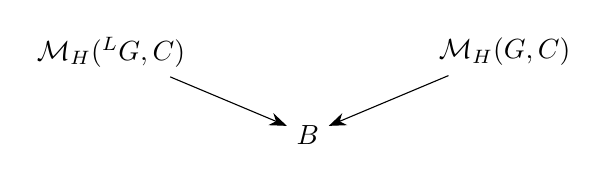
\begin{tikzpicture}[>={Stealth[length=2.2mm]},scale=1.0]
  \node (L) at (0,1.05) {$\MH(\LG,C)$};
  \node (G) at (5.0,1.05) {$\MH(G,C)$};
  \node (B) at (2.5,0) {$B$};
  \draw[->] (L) -- (B);
  \draw[->] (G) -- (B);
\end{tikzpicture}
\caption{Hitchin 纤维化：$G$ 与对偶群 $\LG$ 的解空间以同一个底 $B$ 为底。（原文第 4 页以文字排出的示意图，此处重排为图形，内容未变。）}
\label{fig:hitchin}
\end{figure}

在复结构 $I$ 下，一般点 $b\in B$ 上的纤维粗略地说是对偶阿贝尔簇（更准确地说，是对偶阿贝尔簇上的 torsor）。换一个角度，这些纤维是辛结构 $\omega=\omega_{K}$ 下的特殊拉格朗日子流形。从后一角度看，同一幅图给出的是 $\MH(\LG,C)$ 在复结构 $J$ 下的 B-模型与 $\MH(G,C)$ 以辛结构 $\omega_{K}$ 的 A-模型之间的镜像对称。

正如我们刚刚解释的，使这一镜像对称显露出来的工具，是 $\MH$ 的超凯勒结构及其 Hitchin 纤维化。这些结构依赖于 $C$ 上复结构的选择，但事实上所得的镜像对称并不真正依赖这一选择\zhnt{3.6}。这一点是在 Kapustin 与 Witten (2007) 中、在从四维拓扑场论导出这一镜像对称例子的过程中被证明的。这里所说的拓扑场论，由 $\mathcal{N}=4$ 超 Yang–Mills 理论经扭转得到。

\subsection{几点提示}

要从这个镜像对称的例子走到几何 Langlands 对偶的通常表述，还有几个障碍要克服。遗憾的是，此处不便多谈，只能给出几点提示。

一个要点是：在通常的表述中，$\MH(\LG,C)$ 上一个 B-膜的对偶，应当不是 $\MH(G,C)$ 上的 A-膜——而那恰恰是我们从上述构造中最自然地得到的东西——而是 $M(G,C)$（$C$ 上 $G$-丛的模空间）上的 D-模层（所谓 D-模层，按定义就是 $M(G,C)$ 上微分算子层 $\mathcal{D}$ 的模层）\zhnt{3.7}。这两种陈述之间的联系在 Kapustin 与 Witten (2007) 第 11 节中得到解释，用到了 $\MH(G,C)$ 上一个特殊的 A-膜，它与 $M(G,C)$ 上的微分算子有密切关系。这种联系之所以可能，是因为如 Hitchin (1987a) 所述，$\MH(G,C)$ 以 $T^{*}M_{\mathrm{st}}(G,C)$ 作为一个 Zariski 开集；这里 $M_{\mathrm{st}}(G,C)$ 是 $M(G,C)$ 中参数化严格稳定丛的子空间。

另一个要点如下。在通常的表述中，几何 Hecke 算子起着核心作用，它们作用在 $C$ 上的全纯 $G$-丛上，因而也作用在 $M(G,C)$ 上的 D-模上。它们在这一图景中有其自然的位置，但正是在这里，若只试图用二维 $\sigma$ 模型与镜像对称来表达这一主题，就会漏掉一些东西。这一特定的镜像对称例子实际上源自一个底层四维规范场论中的对偶。一旦理解了这一点，关于规范场论的 Wilson 与 't Hooft 线算子的基本事实就会给出关于 Hecke 特征层的通常陈述，如 Kapustin 与 Witten (2007) 第 9、10 节所解释的那样。几何 Hecke 算子在这一语境中自然地用三维规范场论的 Bogomolny 方程重新解释；这些方程在几何上与物理上都极有意义，并已被大量研究，例如见 Atiyah 与 Hitchin (1988)\zhnt{3.8}。

这些陈述中的某一些若要得到恰当的表述，就会引出四维的另一个重要作用。几何 Langlands 的通常表述所涉及的 D-模，不是在半稳定 $G$-丛的模空间上，而是在所有 $G$-丛的模叠上。主要原因是：若只考虑半稳定丛，就看不到 Hecke 算子的作用。正如我们将在第 6 节说明的，叠在标准描述中的这种地位，可以被理解为一条强有力的线索，指向一个从四维规范场论出发的替代进路。

% =====================================================================
%  sec4.tex — 4. Ramification
%  原文 pp.5–7
% =====================================================================
\section{分歧}

不过，在回到叠之前，我想先说明一下几何 Langlands 语境中所谓的「分歧」是什么意思。

对我们迄今所说的内容，一个简单的推广是：考虑的不是闭的定向二维流形 $C$ 上的平坦丛，而是带穿刺点的二维流形 $C'=C\setminus p$ 上的平坦丛；也就是说，$C'$ 是从 $C$ 中挖去一点 $p$ 而得到的\zhnt{4.1}。

我们选取一个共轭类 $\mathcal{C}\subset G_{\C}$，并记 $\YC(G,C';\mathcal{C})$ 为同态 $\rho:\pi_{1}(C')\to G_{\C}$ 的模空间（模去共轭），要求绕 $p$ 的单值性落在共轭类 $\mathcal{C}$ 中\zhnt{4.2}。

我们以前作过的许多陈述，在这种带穿刺点的情形下都有自然的类比。特别地，$\YC(G,C';\mathcal{C})$ 具有复辛流形的自然结构：它有自然的复结构与全纯辛形式 $\Omega$。与无穿刺点的情形一样，我们可以定义 $\YC(G,C';\mathcal{C})$ 的 B-模型；同时，把 $\YC(G,C';\mathcal{C})$ 看作以 $\omega=\operatorname{Im}\Omega$ 为辛形式的实辛流形，我们也可以定义 A-模型。B-模型与 A-模型都完全不依赖 $C'$ 的复结构。

其次，引入对偶群 $\LG$，并令 ${}^{L}\mathcal{C}$ 为其复化中的一个共轭类。同样，空间 $\YC(\LG,C';{}^{L}\mathcal{C})$ 有自然的 B-模型与 A-模型。

基于我们迄今所说的，人们或许会猜想：对 $\mathcal{C}$ 与 ${}^{L}\mathcal{C}$ 之间的某个映射，$\YC(G,C';\mathcal{C})$ 与 $\YC(\LG,C';{}^{L}\mathcal{C})$ 之间可能存在镜像对称。这个问题的答案是「不完全是」，原因有几条。一个问题是：$G_{\C}$ 中的共轭类与 ${}^{L}G_{\C}$ 中的共轭类之间没有自然的对应。更根本的问题是：$\YC(G,C';\mathcal{C})$ 的 B-模型全纯地依赖于共轭类 $\mathcal{C}$，而同一空间的 A-模型却不\zhnt{4.3}。要找到一种有可能正确的陈述形式，我们必须添加额外的参数，才能得到一个镜像对称的参数组。

无论如何，不管添加什么参数，只要把 $C'$ 仅看成一个带穿刺点的定向二维流形，镜像对称的问题就极难回答。为了取得进展，正如在非分歧情形（即无穿刺点的情形）中那样，给 $C'$ 配上一个复结构并使用 Hitchin 方程是非常有帮助的。这实际上也帮助我们找到正确的参数：在试图给带穿刺点曲面上的 Hitchin 方程一个自然表述时，一套改进了的参数就出现了。设 $z$ 是穿刺点附近的局部参数，写作 $z=re^{i\theta}$。在带穿刺点的情形，自然地（见 Simpson 1990）引入取值于极大环面 $T\subset G$ 的李代数 $\mathfrak{t}$ 的变量 $\alpha,\beta,\gamma$，并考虑 $C'$ 上 Hitchin 方程的解，使其在 $z=0$ 附近的行为如下：
\begin{equation}
A=\alpha\,d\theta+\cdots
\label{eq:A-asym}
\end{equation}
\begin{equation}
\phi=\beta\,\frac{dr}{r}-\gamma\,d\theta+\cdots.
\label{eq:phi-asym}
\end{equation}
省略号指在 $z=0$ 附近奇性更弱的项\zhnt{4.4}。

关于 Hitchin 方程的一切通常陈述，在这种情形下都有密切的类比。以这种奇性为奇性的 Hitchin 方程之解的模空间，是一个超凯勒流形 $\MH(G,C;\alpha,\beta,\gamma)$。在其中一个复结构（通常记作 $J$）下，它与 $\YC(G,C;\mathcal{C})$ 一致，其中 $\mathcal{C}$ 是包含 $U=\exp(-2\pi(\alpha-i\gamma))$ 的共轭类\yz{为简单起见，我们假定 $U$ 是正则的。一般情形下成立的、更为复杂的陈述见 Gukov 与 Witten (2006)。}\zhnt{4.5}。在另一个复结构（常记作 $I$）下，$\MH(G,C;\alpha,\beta,\gamma)$ 参数化 Higgs 丛 $(E,\varphi)$，其中 $\varphi\in H^{0}(C',K\otimes\ad(E))$ 在 $z=0$ 处有极点，且
\[
\varphi\sim\tfrac12(\beta+i\gamma)\,(dz/z).
\]
此外还有 Hitchin 纤维化，并且非分歧情形的大部分通常陈述——既包括我们已解释过的，也包括此处省略未讲的——都有密切的类比。更详细的解释以及对原始文献的指引，见 Gukov 与 Witten (2006)。

变量 $\alpha,\beta,\gamma$ 是经典几何的一套自然参数。然而在量子层面，还有一个自然变量 $\eta$（类似于规范场论中通常的 $\theta$-角），如 Gukov 与 Witten (2006) 第 2.3 节所述。有了完整的参数组 $(\alpha,\beta,\gamma,\eta)$，就有可能表述一个自然的对偶陈述：$\MH(\LG,C;{}^{L}\alpha,{}^{L}\beta,{}^{L}\gamma,{}^{L}\eta)$ 镜像于 $\MH(G,C;\alpha,\beta,\gamma,\eta)$，参数之间有某个映射，见 Gukov 与 Witten (2006) 第 2.4 节。这个映射的要点是 $(\alpha,\eta)=({}^{L}\eta,-{}^{L}\alpha)$\zhnt{4.6}。由于单值性 $U$ 依赖于 ${}^{L}\alpha$，这就说明：单值性的对偶涉及量子参数 $\eta$，而后者在经典几何中是看不见的。在 A-模型中，$\eta$ 成为复化 Kähler 类的虚部。

这一对偶陈述在再次把 A-膜对应到 D-模之后，给出这一情形下几何 Langlands 对偶的一个陈述，与 Frenkel 与 Gaitsgory (2005) 中通过代数几何与二维共形场论所得的结果类似。

\begin{remark}
我们在此停下，解释关于经典几何的一个很基本的事实，它可作为第 5 节的背景。在复结构 $J$ 下，具有式 \eqref{eq:A-asym} 那种奇性的 Hitchin 方程之解，描述一个平坦 $G_{\C}$-丛 $E\to C'$，其绕穿刺点 $p$ 有单值性。$E$ 可以延拓过 $p$ 成为一个全纯丛，当然不能延拓为平坦丛；而且，从全纯的观点看，$E$ 在 $p$ 附近可以被平凡化。于是 $E\to C'$ 上的平坦联络在这一规范下，由 $C'$ 上的一个全纯 $(1,0)$-形式（取值于 $G_{\C}$ 的李代数）表示，该形式在 $p$ 处有单极点：
\begin{equation}
A=dz\left(\frac{\alpha-i\gamma}{iz}+\cdots\right),
\label{eq:regular}
\end{equation}
其中省略的项在 $z=0$ 处正则。联络在 $z=0$ 处的奇性之所以是单极点，是因为 Hitchin 方程的拟设 \eqref{eq:A-asym} 只允许 $1/|z|$ 阶的奇性。具有这种单极点的全纯联络，称为有正则奇点\zhnt{4.7}。

在几何 Langlands 中，通常所谓的驯顺分歧，粗略地说就是我们刚刚到达的情形：全纯丛 $E\to C$ 带有一个有正则奇点的全纯联络形式。其实，「驯顺分歧」这个说法有时被用来指单极点的留数是幂零的情形，而在式 \eqref{eq:regular} 中我们似乎处在相反的情形，即半单留数。Gukov 与 Witten (2006) 中说明：只要稍加小心，$\MH(G,C';\alpha,\beta,\gamma,\eta)$ 的镜像对称实际上就是一个足够好的框架，可以理解任意留数的单极点情形下的几何 Langlands。例如，幂零留数的情形可以通过令 ${}^{L}\alpha={}^{L}\gamma=0$（或在对偶描述中令 $\gamma=\eta=0$）来理解。
\end{remark}

% =====================================================================
%  sec5.tex — 5. Wild Ramification
%  原文 pp.7–10
% =====================================================================
\section{野分歧}

基于与数论的类比，几何 Langlands 通常并不只对驯顺分歧的情形表述。人们会进一步追问一个类似的、涉及带有任意阶极点处的全纯联络的丛 $E\to C$ 的对偶陈述。换言之，在把 $E$ 在一个点 $p\in C$ 附近的全纯结构平凡化之后，联络看起来像
\begin{equation}
A=dz\left(\frac{T_{n}}{z^{n}}+\frac{T_{n-1}}{z^{n-1}}+\cdots+\frac{T_{1}}{z}+\cdots\right),
\label{eq:wild}
\end{equation}
其中正则项被省略。极点阶数大于 $1$ 的亚纯联络，称为有非正则奇点。

要为此情形表述一个对偶陈述，乍看之下对此处所述的几何 Langlands 进路构成严峻挑战。我们的基本观点是：那些根本的对偶陈述只依赖 $C$ 作为一个定向二维流形。$C$ 上的复结构只是作为一种工具被引入，用来回答某些在不引入复结构的情况下也能提出的自然问题。

从这个观点看，驯顺分歧是自然的，因为这种意义上的单极点有清楚的拓扑含义。在点 $p\in C$ 处有单极点的亚纯联络，是编码 $C'=C\setminus p$ 上平坦联络绕 $p$ 的单值性的一种自然方式。而这一单值性当然是纯粹拓扑的概念。然而，一个阶数大于 $1$ 的极点，其拓扑含义可能是什么呢？

一个密切相关的观察是：$T_{1}$ 是 $A$ 在 $z=0$ 处极点的留数\zhnt{5.1}，因而与局部坐标 $z$ 的选择无关。然而高阶极点的系数 $T_{2},\dots,T_{n}$ 却肯定依赖于局部坐标的选择\zhnt{5.2}。我们怎能希望把它们纳入一个只应依赖 $C$ 作为定向二维流形的理论呢？

而且，如果计划是先表述一个拓扑性质的对偶猜想、再用 Hitchin 方程去证明它，那么我们就要面对 Hitchin 方程是否与非正则奇点相容的问题。关于对 $\Phi=(A,\phi)$ 的 Hitchin 方程，其形式概略地说是 $d\Phi+\Phi^{2}=0$。若在 $z=0$ 附近奇性满足 $|\Phi|\sim1/|z|^{n}$，则 $|d\Phi|\sim1/|z|^{n+1}$，而 $|\Phi|^{2}\sim1/|z|^{2n}$。当 $n=1$ 时，$d\Phi$ 与 $|\Phi|^{2}$ 量级相当，因此 Hitchin 方程看起来是合理的。然而当 $n>1$ 时，$|\Phi|^{2}\gg|d\Phi|$，Hitchin 方程中的非线性项看来会太强\zhnt{5.3}。

不过，两个问题都有自然的答案。对第一个问题的答案是：尽管表面上不然，人们确实可以给非正则奇点的联络关联上某种超出普通单值性、且具有纯拓扑含义的东西。恰当的概念是扩张单值性，它既包含 Stokes 矩阵，也包含普通单值性。Stokes 矩阵是常微分方程非正则奇点经典理论的一部分，例如见 Wasow (1965)\zhnt{5.4}。

为简洁起见，假定联络奇异部分的首项系数 $T_{n}$ 是正则半单的，那么可以作一个规范变换，把 $T_{1},\dots,T_{n}$ 共轭到极大环面中。然后定义模空间 $\YC(G,C;T_{1},\dots,T_{n})$，它在规范变换下参数化这样的对：$C$ 上的全纯 $G_{\C}$-丛，以及一个具有式 \eqref{eq:wild} 所述非正则奇点的联络。如 Boalch (2001) 所证明，这个空间 $\YC(G,C;T_{1},\dots,T_{n})$ 自然地是一个复辛流形，其复辛结构只依赖 $C$ 作为定向二维流形。这一点可以通过把 Atiyah 与 Bott (1982) 中表述的辛结构的规范场论定义搬到当前情形来证明。

此外，$\YC(G,C;T_{1},\dots,T_{n})$ 的复辛结构与 $T_{2},\dots,T_{n}$ 无关（只要 $T_{n}$ 保持半单）。

此时，Jimbo 等 (1981) 引入的重要概念——等单值形变——就登场了。存在一种自然的方式改变参数 $T_{2},\dots,T_{n}$，而不改变由 $\YC(G,C;T_{1},\dots,T_{n})$ 所参数化的广义单值数据。而且，如 Boalch (2001) 新近证明的，广义单值数据空间的复辛结构在等单值形变下不变\zhnt{5.5}。于是粗略地说，可以定义一个只依赖 $T_{1}$ 与整数 $n\ge1$ 的复辛流形 $\YC(G,C;T_{1},n)$。

参数 $T_{2},\dots,T_{n}$ 按刚才所述的意义是非本质的，这当然是受欢迎的，因为正如我们已经注意到的，它们没有明显的拓扑含义。现在我们处在与非分歧、驯顺分歧情形非常相似的局面中。给定复辛流形 $\YC(G,C;T_{1},n)$ 及其复辛形式 $\Omega$，我们可以定义它的 B-模型，或者用实辛形式 $\omega=\operatorname{Im}\Omega$ 定义它的 A-模型。当然，对偶群也可以同样处理，定义另一个复辛流形 $\YC(\LG,C;{}^{L}T_{1},n)$，及其自己的 B-模型与 A-模型。而正如非分歧情形一样，我们可以问这两个模型是否互为镜像。

甚至在尝试回答这个问题之前，我们应先把问题稍作精细化。由于要求 $T_{n}$ 是正则半单的，简单地把 $T_{n}$ 忘掉并不完全正确。当 $T_{n}$ 变化时可能有单值性。我们把 $T_{n}$ 看作取值于 $\mathfrak{t}_{\C}^{\mathrm{reg}}\otimes K_{p}^{n-1}$，记号如下：$\mathfrak{t}_{\C}$ 是 $G_{\C}$ 中极大环面的李代数，$\mathfrak{t}_{\C}^{\mathrm{reg}}$ 是其中由正则元构成的子空间，$K_{p}$ 是 $C$ 的余切丛在 $p$ 处的纤维。$\mathfrak{t}_{\C}^{\mathrm{reg}}$ 的基本群称为 $G$ 的辫群；我们记之为 $B(G)$\zhnt{5.6}。由于这些单值性，为了定义 $\YC(\LG,C;{}^{L}T_{1},n)$，实际上需要选取基点 $*\in\mathfrak{t}_{\C}^{\mathrm{reg}}$；更精确地说，我们可以把这个空间记作 $\YC(\LG,C;{}^{L}T_{1},n,*)$。群 $B(G)$ 通过单值性同时作用在 $\YC(G,C;T_{1},n,*)$ 的 B-模型与 A-模型上。对偶地，相应的辫群 $B(\LG)$ 作用在 $\YC(\LG,C;{}^{L}T_{1},n,*)$ 的 B-模型与 A-模型上。

然而，$B(G)$ 与 $B(\LG)$ 这两个群自然同构；确实，模去一个不变二次型的选择，存在从 $\mathfrak{t}_{\C}^{\mathrm{reg}}$ 到 ${}^{L}\mathfrak{t}_{\C}^{\mathrm{reg}}$ 的自然映射，因此这两个空间有相同的基本群，且其中一个中基点的选择（在同伦意义下）决定了另一个中的基点。一个更好（但仍不精确）的问题是：$\YC(G,C;T_{1},n,*)$ 与 $\YC(\LG,C;{}^{L}T_{1},n,*)$ 之间是否存在一个与辫群作用交换的镜像对称。

我们还期待这一镜像对称只依赖 $C$ 作为定向二维流形，从而与映射类群交换。我们可以把 $C$ 的映射类群与辫群看作扮演相当平行的角色。事实上，由于上一段中典范丛的纤维 $K_{p}$ 的出现，这两个群并不只是彼此交换；作用着的群是映射类群被 $B(G)$ 的一个扩张\zhnt{5.7}。

正如驯顺分歧情形一样，要得到正确的镜像对称猜想，我们需要把参数稍作扩充，以得到一个镜像对称的参数组。但我们也面对 Hitchin 方程是否与野分歧相容这一根本问题。如上所述，Hitchin 方程的非线性使这一点乍看可疑。但幸运的是，结果表明一切正常，如 Biquard 与 Boalch (2004) 所证明。要点是：同样在假定 $T_{n}$ 正则半单的前提下，我们可以假定联络的奇异部分是交换的。Hitchin 方程虽然非线性，在交换情形下却变成线性的；而一旦交换化，它们就与任意阶的奇性相容。以此出发，结果表明对任何 $n$ 都可以发展出一套与非分歧情形中更熟悉的故事相当平行的、带非正则奇点的 Hitchin 方程理论。例如，方程解的模空间 $\MH$ 是超凯勒的。在其中一个复结构下，$\MH$ 参数化具有类似式 \eqref{eq:wild} 那种奇性的平坦联络；在另一个复结构下，它参数化 Higgs 丛 $(E,\phi)$，其中 $\phi$ 有阶数为 $n$ 的类似极点。存在 Hitchin 纤维化，所有通常的性质都有密切的类比。

这一切恰好给出了正确的素材，可用 Hitchin 方程来建立这两个模空间之间所期望的镜像对称。详细的解释（其中这一经典几何被嵌入四维规范场论）见 Witten (2007)。许多论证与前面给出的论证相当类似。

% =====================================================================
%  sec6.tex — 6. Four-Dimensional Gauge Theory And Stacks（含 6.1 Stacks）
%  原文 pp.10–14
% =====================================================================
\section{四维规范场论与叠}

对物理学家来说，在研究涉及规范场论的对偶时，从四维开始是自然的，因为四维常被发现是规范场论对偶的自然舞台。理由很简单：曲率——规范场论中最基本的概念之一——是一个 2-形式；在 $d$ 维中，2-形式的对偶是 $(d-2)$-形式，所以只有当 $d=4$ 时它仍然是 2-形式\zhnt{6.1}。这提示 $d=4$ 是「一个规范场论的对偶可能仍是规范场论」的最自然的维数。

此外，$\mathcal{N}=4$ 超对称 Yang--Mills 理论（最初由 Brink 等 (1977) 构造）是自然的起点，因为它具有可能的最大超对称，并拥有可追溯到 Montonen 与 Olive (1977) 早期工作的著名对偶\zhnt{6.2}。结果确实如此：几何 Langlands 在四维 $\mathcal{N}=4$ 超 Yang--Mills 理论的一个扭转版本中有其自然的起源。这种扭转与导致 Donaldson 理论的 $\mathcal{N}=2$ 超 Yang--Mills 理论的扭转相当类似。

那个特定的动机对某些人来说可能晦涩；因此，为理解几何 Langlands，我在这里改用另一种方式来解释为什么从四维开始是自然的，而不是只依赖 $\MH(G,C)$ 的 B-模型与 A-模型。

首先，任何空间 $X$ 的 B-模型与 A-模型，都是支配映射 $\Phi:\Sigma\to X$ 的量子 $\sigma$ 模型的扭转版本，其中 $\Sigma$ 是一个二维流形（更确切地说，是一个玻色维数为 2 的超流形）\zhnt{6.3}。由于 A-模型在其最基本的形式中涉及对满足适当条件的全纯映射 $\Phi:\Sigma\to X$ 的计数，$\Sigma$ 与 $\Phi$ 在 A-模型中的角色是清楚的。镜像对称表明，用映射 $\Phi:\Sigma\to X$ 来表述 B-模型也必定是正确的，而物理学家在通常的表述中正是这样做的。

在目前的情形中，我们粗略地说对某个紧 Lie 群 $G$ 与二维流形 $C$ 的空间 $\MH(G,C)$ 的 B-模型与 A-模型感兴趣。因此粗略地说，我们想研究映射 $\Phi:\Sigma\to\MH(G,C)$ 的 $\sigma$ 模型，其中如前 $\Sigma$ 是一个辅助的二维流形。

这一描述之所以粗略，是因为 $\MH(G,C)$ 有奇点\yz{此外，这些奇点比轨形奇点更坏。轨形奇点不会造成任何困难。关于几何 Langlands 中轨形奇点的讨论，见 Frenkel 与 Witten (2007)。}，因此以 $\MH(G,C)$ 为目标的 $\sigma$ 模型并非真正良定义。所以，一个完整的描述不能纯粹用「目标空间是视为抽象流形的 $\MH(G,C)$」的 $\sigma$ 模型来给出。我们需要一个更完整的描述，告诉我们如何处理这些奇点。这会是什么呢？

按定义，$\MH(G,C)$ 中的一个点在规范等价下决定一个满足 Hitchin 方程的对 $(A,\phi)$。$A$ 与 $\phi$ 是定义在 $C$ 上的场，所以我们把它们更明确地写成 $(A(y),\phi(y))$，其中 $y$ 是 $C$ 上的坐标。

现在设有一个映射 $\Phi:\Sigma\to\MH(G,C)$，其中 $\Sigma$ 是带局部坐标 $x$ 的黎曼面。这样的映射由一对同时依赖 $x$ 的 $(A(y),\phi(y))$ 描述。于是我们可以用同时依赖 $x$ 与 $y$ 的场 $(A(x,y),\phi(x,y))$ 来描述映射 $\Phi$。我们希望把这些场解释为四维流形 $M=\Sigma\times C$ 上的场\zhnt{6.4}。对 $(A(x,y),\phi(x,y))$ 并不完全是一组 $M$ 上的自然场，但可以自然地补全为这样一组。例如，$A(x,y)$ 局部地是切于 $M=\Sigma\times C$ 中第二个因子的 1-形式；要得到四维规范场，我们应放松 $A$ 切于第二个因子这一条件。类似地，我们可以把 $\phi$ 延拓为 $\Sigma\times C$ 上取值于伴随丛的 1-形式。$\mathcal{N}=4$ 超 Yang--Mills 理论——更确切地说，与几何 Langlands 相关的它的扭转版本——正是通过以最小方式把这组场补全为一个超对称组合而得到的。

在 $\mathcal{N}=4$ 超 Yang--Mills 理论中，没有类似于 $\MH(G,C)$ 的奇点。例如，规范场的空间是仿射空间，其他场（如 $\phi$）取值于线性空间。使「映射 $\Phi:\Sigma\to\MH(G,C)$ 的 $\sigma$ 模型」难以定义的那些奇点问题，在 $M=\Sigma\times C$（或任何其他四维流形）上定义规范场论时都没有类似物。两者的关系是：二维 $\sigma$ 模型是四维规范场论的近似\zhnt{6.5}。当遇到 $\MH(G,C)$ 的奇点时，这一近似失效。任何涉及这些奇点的问题，都应在底层的四维规范场论中处理。

不过，远离奇点时，只需考虑描述映射 $\Phi:\Sigma\to\MH(G,C)$ 的那组较小的场就够了。许多问题不依赖奇点，对这些问題，用二维 $\sigma$ 模型与镜像对称来描述是足够的。

\subsection{叠}

作为结论，我们将与上述讨论在通常的数学理论中的对应物建立联系。我们从丛而不是 Higgs 丛开始，因为这一情形更容易解释。

在通常的数学理论中，几何 Langlands 对应的右手边是用 D-模来描述的，粗略地说，是在黎曼面 $C$ 上所有全纯 $G_{\C}$-丛的模空间上。然而，人们考虑的不是半稳定全纯 $G_{\C}$-丛 $E\to C$ 的模空间 $M(G,C)$，而是所有这类丛的「叠」$\Bun_{G}(C)$ 上的 D-模\zhnt{6.6}。主要原因是：要定义 Hecke 算子的作用，就必须允许不稳定丛。不稳定丛与 $M(G,C)$ 的非轨形奇点有关。

什么是叠？粗略地说，它是一个可以处处局部地描述为商的空间。平凡的情形是：一个叠实际上可以整体地描述为商。把 $\Bun_{G}(C)$ 解释为整体商，意味着要找一对 $(Y,W_{\C})$，由一个光滑代数簇 $Y$ 与一个作用在 $Y$ 上的复 Lie 群 $W_{\C}$ 组成，具有以下性质：全纯 $G_{\C}$-丛 $E\to C$ 的同构类应与 $Y$ 上的 $W_{\C}$-轨道一一对应；并且对每个 $E\to C$，其自同构群应同构于 $W_{\C}$ 中固定 $Y$ 中对应点的子群。

如果要求 $Y$ 与 $W_{\C}$ 是有限维的，那么以此方式表示叠 $\Bun_{G}(C)$ 的对 $(Y,W_{\C})$ 并不存在\zhnt{6.7}。确实，$G_{\C}$-丛 $E\to C$ 可以任意不稳定，所以其自同构群的维数没有上界。因此没有有限维的 $W_{\C}$ 能包含所有这些自同构群作为子群。

然而正如 Atiyah 与 Bott (1982) 所证明的，为简单起见取 $G$ 为伴随型，存在自然的无穷维对 $(Y,W_{\C})$。只需取 $Y$ 为给定（最初只在拓扑上定义的）$G$-丛 $E\to C$ 上所有联络的空间。定义 $W$ 为丛 $E$ 的所有规范变换构成的群；于是若 $E$ 拓扑平凡，可把 $W$ 等同于 $\Maps(C,G)$。然后取 $W_{\C}$ 为 $W$ 的复化，换言之 $\Maps(C,G_{\C})$。（这个复化如下作用在 $Y$ 上：把联络 $A$ 对应到相应的 $\bar\partial$ 算子 $\bar\partial_{A}$；于是复值规范变换按 $\bar\partial_{A}\to g\bar\partial_{A}g^{-1}$ 作用。）

设我们被摆在这样的问题面前：已知 $M(G,C)$ 的奇点，要弄清映射 $\Phi:\Sigma\to M(G,C)$ 的超对称 $\sigma$ 模型的含义。（这是我们真正问题——涉及 $\MH(G,C)$ 而不是 $M(G,C)$——的一个练习情形。）代数几何方面的朋友会告诉我们用叠 $\Bun_{G}(C)$ 替换 $M(G,C)$。我们把这一叠解释为对 $(Y,W_{\C})$，其中 $Y$ 是 $G$-丛 $E\to C$ 上所有联络的空间，$W_{\C}$ 是复化的规范变换群。叠的连通分支对应 $E$ 的拓扑选择。

所谓以一对 $(Y,W_{\C})$（$W_{\C}$ 是作用在复流形 $Y$ 上的复 Lie 群）为目标的超对称 $\sigma$ 模型，在有限维情形下，我们指的是规范群为 $W$（$W_{\C}$ 的极大紧子群）、目标为 $Y$ 的规范不变超对称 $\sigma$ 模型。实际上，要定义这个 $\sigma$ 模型，我们希望 $Y$ 是一个带 $W$-不变（当然不是 $W_{\C}$-不变）Kähler 结构的 Kähler 流形。$\sigma$ 模型作用量含有一项，它是 $W$ 作用的矩映射的平方。这一项恰在矩映射为零时取极小。把矩映射置零并对 $W$ 取商，这二者合起来在经典上等价于对 $W_{\C}$ 取商\zhnt{6.8}。

要写下作用量中涉及矩映射平方的那一项（事实上，要写下规范场的动能项），需要在 $W$ 的李代数上有一个不变正定二次型。若 $W$ 是有限维的，这种形式的存在等价于 $W$ 是紧的\zhnt{6.9}。然而在 $W=\Maps(C,G)$（对某个空间 $C$）的无穷维情形中，相应的二次型也存在。（$W$ 的李代数的一个元素是 $C$ 上取值于 $\mathfrak{g}$ 的函数 $\epsilon$，二次型由 $\int_{C}d\mu\,(\epsilon,\epsilon)$ 定义，其中 $(\ ,\ )$ 是 $\mathfrak{g}$ 上不变正定二次型，$\mu$ 是 $C$ 上适当的测度。）

现在，设我们构造从黎曼面 $\Sigma$ 到叠 $\Bun_{G}(C)$ 的映射的二维 $\sigma$ 模型，叠按上述方式理解。这个 $\sigma$ 模型的规范变换群是什么？一般地，在任何空间 $\Sigma$ 上规范群为 $W$ 的规范场论中，规范变换群（为简单起见，取拓扑平凡 $W$-丛的）是从 $\Sigma$ 到 $W$ 的映射群，即 $\Maps(\Sigma,W)$。在我们的情形，$W$ 又是 $\Maps(C,G)$。所以 $\Maps(\Sigma,W)$ 就是 $\Maps(M,G)$，其中 $M=\Sigma\times C$。但这正是 $M$ 上规范群为 $G$ 的规范场论中的规范变换群。在目前情形，$\Sigma$ 与 $C$ 是二维流形，$M$ 是四维流形。我们已经到达四维规范场论。若把定义再追问得细一些，我们就会知道：映射 $\Phi:\Sigma\to\Bun_{G}(C)$ 的超对称 $\sigma$ 模型应被理解为四维流形 $M=\Sigma\times C$ 上规范群为 $G$ 的四维 $\mathcal{N}=2$ 超对称规范场论。（这是扭转后与 Donaldson 理论相关的那套理论。）

现在回到原来的问题。几何 Langlands 对偶是关于 $\MH(G,C)$（相应的 Higgs 丛模空间）及其对偶群版本 $\MH(\LG,C)$ 的 B-模型与 A-模型的陈述，而不是关于 $M(G,C)$ 的。为处理奇点，我们想把这一情形「叠化」。我们现在处在超凯勒的语境中，叠的恰当概念应把这一点纳入。（代数几何家所谓的 Higgs 丛的叠并不足以胜任这一情形，因为它过于强调一个复结构。）由于四元数 Lie 群不存在，我们不能要求把 $\MH(G,C)$ 构造为光滑空间被四元数 Lie 群取商\zhnt{6.10}。然而，辛商的概念在超凯勒世界中有很好的类比，即 Hitchin 等 (1987) 所描述的超凯勒商。对我们为 $M(G,C)$ 所解释的东西的类比是：把 $\MH(G,C)$ 实现为光滑空间 $Y$ 被群 $W$ 的超凯勒商。用有限维的 $Y$ 与 $W$ 来做这件事可能做不到，但在无穷维世界中，这个问题在 Hitchin 关于 Hitchin 方程的原始论文 Hitchin (1987a) 中有一个自然的解。（$Y$ 是 $C$ 上对 $(A,\phi)$ 的空间，$W=\Maps(C,G)$。）以此为输入，并解释「目标为对应于 $\MH(G,C)$ 的超凯勒叠的 $\sigma$ 模型」应当意味着什么，人们就得到 $\mathcal{N}=4$ 超 Yang--Mills 理论的扭转版本——而这也正是 Kapustin 与 Witten (2007) 的出发点。


\clearpage
% =====================================================================
%  refs.tex — References（原文 pp.14–15）
%  文献条目依原文照录，仅整理断行；未作任何增删。
% =====================================================================
\phantomsection
\addcontentsline{toc}{section}{参考文献}

\begin{thebibliography}{99}\small

\bibitem[AB82]{AtiyahBott1982}
M.~F. Atiyah and R.~Bott,
\newblock The Yang--Mills equations over Riemann surfaces,
\newblock \emph{Phil. Trans. Roy. Soc. London} \textbf{A308} (1982), 166--186.

\bibitem[AH88]{AtiyahHitchin1988}
M.~F. Atiyah and N.~J. Hitchin,
\newblock \emph{The Physics and Geometry of Monopoles},
\newblock Princeton University Press, 1988.

\bibitem[BJSV95]{Bershadsky1995}
M.~Bershadsky, A.~Johansen, V.~Sadov and C.~Vafa,
\newblock Topological reduction of $4$-$D$ SYM to $2$-$D$ sigma models,
\newblock \emph{Nucl. Phys.} \textbf{B448} (1995), 166--186.

\bibitem[BB04]{BiquardBoalch2004}
O.~Biquard and P.~Boalch,
\newblock Wild non-abelian Hodge theory on curves,
\newblock \emph{Compos. Math.} \textbf{140} (2004), 179--204.

\bibitem[Boa01]{Boalch2001}
P.~Boalch,
\newblock Symplectic manifolds and isomonodromic deformations,
\newblock \emph{Adv. Math.} \textbf{163} (2001), 137--205.

\bibitem[BSS77]{Brink1977}
L.~Brink, J.~H. Schwarz and J.~Scherk,
\newblock Supersymmetric Yang--Mills theories,
\newblock \emph{Nucl. Phys.} \textbf{B121} (1977), 77.

\bibitem[FG05]{FrenkelGaitsgory2005}
E.~Frenkel and D.~Gaitsgory,
\newblock Local geometric Langlands correspondence and affine Kac--Moody algebras,
\newblock \texttt{math.RT/0508382}.

\bibitem[FW07]{FrenkelWitten2007}
E.~Frenkel and E.~Witten,
\newblock Geometric endoscopy and mirror symmetry,
\newblock to appear.

\bibitem[Gua03]{Gualtieri2003}
M.~Gualtieri,
\newblock Generalized complex geometry,
\newblock D.~Phil. Thesis, Oxford University, \texttt{math.DG/0401221}.

\bibitem[GW06]{GukovWitten2006}
S.~Gukov and E.~Witten,
\newblock Gauge theory, ramification, and the geometric Langlands program,
\newblock \texttt{hep-th/0612073}.

\bibitem[HMS95]{Harvey1995}
J.~A. Harvey, G.~W. Moore and A.~Strominger,
\newblock Reducing $S$ duality to $T$ duality,
\newblock \emph{Phys. Rev.} \textbf{D52} (1995), 7161--7167.

\bibitem[HT02]{HauselThaddeus2002}
T.~Hausel and M.~Thaddeus,
\newblock Mirror symmetry, Langlands duality, and the Hitchin system,
\newblock \texttt{math.AG/0205236}.

\bibitem[Hit87a]{Hitchin1987a}
N.~J. Hitchin,
\newblock The self-duality equations on a Riemann surface,
\newblock \emph{Proc. London Math. Society} (3) \textbf{55} (1987), 67.

\bibitem[Hit87b]{Hitchin1987b}
N.~J. Hitchin,
\newblock Stable bundles and integrable systems,
\newblock \emph{Duke Math. J.} \textbf{54} (1987), 91--114.

\bibitem[Hit03]{Hitchin2003}
N.~J. Hitchin,
\newblock Generalized Calabi--Yau manifolds,
\newblock \emph{Q. J. Math.} \textbf{54} (2003), 281--308; \texttt{math.DG/0209099}.

\bibitem[HKLR87]{Hitchin1987HKLR}
N.~J. Hitchin, A.~Karlhede, U.~Lindstr\"om and M.~Ro\v{c}ek,
\newblock Hyperk\"ahler metrics and supersymmetry,
\newblock \emph{Commun. Math. Phys.} \textbf{108} (1987), 535--589.

\bibitem[Hori03]{Hori2003}
K.~Hori et al. (eds),
\newblock \emph{Mirror Symmetry},
\newblock American Mathematical Society, Providence, 2003.

\bibitem[JMU81]{Jimbo1981}
M.~Jimbo, T.~Miwa and K.~Ueno,
\newblock Monodromy preserving deformations of linear differential equations with rational coefficients,
\newblock \emph{Physica} \textbf{2D} (1981), 407--448.

\bibitem[KW07]{KapustinWitten2007}
A.~Kapustin and E.~Witten,
\newblock Electric--magnetic duality and the geometric Langlands program,
\newblock \emph{Comm. Number Theory and Physics} \textbf{1} (2007), 1--236; \texttt{hep-th/0604151}.

\bibitem[MO77]{MontonenOlive1977}
C.~Montonen and D.~Olive,
\newblock Magnetic monopoles as gauge particles?,
\newblock \emph{Phys. Lett.} \textbf{B72} (1977), 117.

\bibitem[PS06]{PantevSharpe2006}
T.~Pantev and E.~Sharpe,
\newblock GLSM's for gerbes (and other toric stacks),
\newblock \emph{Adv. Theor. Math. Phys.} \textbf{10} (2006), 77--121; \texttt{hep-th/0502053}.

\bibitem[Sim90]{Simpson1990}
C.~Simpson,
\newblock Harmonic bundles on noncompact curves,
\newblock \emph{J. Am. Math. Soc.} \textbf{3} (1990), 713--770.

\bibitem[SYZ96]{Strominger1996}
A.~Strominger, S.-T. Yau and E.~Zaslow,
\newblock Mirror symmetry is $T$ duality,
\newblock \emph{Nucl. Phys.} \textbf{B479} (1996), 243--259; \texttt{hep-th/9606040}.

\bibitem[Was65]{Wasow1965}
W.~Wasow,
\newblock \emph{Asymptotic Expansions for Ordinary Differential Equations},
\newblock Wiley, New York, 1965.

\bibitem[Wit07]{Witten2007}
E.~Witten,
\newblock Gauge theory and wild ramification,
\newblock \texttt{arXiv:0710.0631}.

\end{thebibliography}

\noindent{\footnotesize
以上条目依原文照录，仅整理断行、补全作者名缩写与刊物卷号格式，未作任何增删。原文中与本篇论证关系最紧的若干条——Atiyah--Bott (1982)、Boalch (2001)、Biquard--Boalch (2004)、Hausel--Thaddeus (2002)、Gukov--Witten (2006)、Kapustin--Witten (2007)、Witten (2007)——在「译者后记」第 4 节按主题作了归并与导读。}


\clearpage
% =====================================================================
%  afterword.tex — 译者后记
%  任务：梳理 Witten 全文的框架与逻辑推导链条（不改动原文，只作导读）
% =====================================================================
\phantomsection
\addcontentsline{toc}{section}{译者后记：这篇文章的骨架与推导链条}
\section*{译者后记：这篇文章的骨架与推导链条}

\subsection*{1. 一句话}

这篇文章要论证的是一件事：\textbf{二维的几何 Langlands 对偶，是四维 $\mathcal{N}=4$ 超对称 Yang--Mills 理论的 S-对偶在某个拓扑扭转之后留下的影子}；而把这两端接起来的桥，是 Hitchin 方程及其纤维化。桥之所以能接通，是因为 Hitchin 纤维化同时具备两种身份：在复结构 $I$ 下它是代数几何里由特征多项式给出的可积系统纤维化，在复结构 $J$ 下它是辛几何里由 $\operatorname{Im}\Omega$ 给出的特殊拉格朗日纤维化，而后者正是 SYZ 意义下的镜像对称\cite{Strominger1996}。于是「两个模空间互为镜像」这句几何上难以直接下手的断言，被换成了「同一个底 $B$ 上的两族对偶环面」这个可以逐纤维验证的陈述\cite{HauselThaddeus2002}。

全文没有证明任何一条新定理。它的价值在于把四组彼此独立发展出来的东西——Hitchin 系统、镜像对称、Montonen--Olive 对偶、几何 Langlands 对应——摆成一个可以互相翻译的框架，并且指出每一处翻译的代价（要添什么参数、要换什么范畴、要放弃什么）。

\subsection*{2. 骨架：六个环节}

原文六节不是并列的六章，而是一条单向的推导链，每一节都在为下一节准备一件不可替代的工具。下图是我们读出的依赖关系；实线是「若不如此，下一节无法开口」的推导依赖，虚线是「回头修正前面定义」的反向依赖。

\begin{figure}[htbp]
\centering
\begin{tikzpicture}[
  box/.style={draw, rounded corners=2pt, align=left, font=\footnotesize,
              text width=7.2cm, inner sep=3.5pt, fill=black!3},
  side/.style={draw, dashed, rounded corners=2pt, align=left, font=\footnotesize,
               text width=4.8cm, minimum height=3.9cm, inner sep=3.5pt, fill=black!3},
  ar/.style={-{Latex[length=2mm]}, semithick},
  dar/.style={-{Latex[length=2mm]}, semithick, dashed},
  lab/.style={font=\scriptsize, fill=white, inner sep=1.2pt, anchor=west, xshift=0.18cm}]

\node[box] (n1) at (0,0)
  {\textbf{\S1}\quad$\YC(G,C)$：平坦 $G_{\C}$-丛的模空间，复辛，$\Omega$ 全纯闭。\\
   两种读法：B-模型（复结构）、A-模型（$\omega=\Imm\Omega$，实辛结构）。};
\node[box, below=1.35cm of n1] (n2)
  {\textbf{\S2}\quad Hitchin 方程 $F-\phi\wedge\phi=0$、$D\phi=D\star\phi=0$；\\
   $J$ 下是 $\YC$，$I$ 下是 Higgs 丛 $\Rightarrow$ $\MH$ 超凯勒。};
\node[box, below=1.35cm of n2] (n3)
  {\textbf{\S3}\quad Hitchin 纤维化 $\MH\to B$：$B$ 由 $\phi$ 的特征多项式决定。\\
   $G$ 与 $\LG$ 同一不变量环 $\Rightarrow$ 同一 $B$，纤维互为对偶阿贝尔簇。\\
   $\Rightarrow$ SYZ：$\MH(G)$ 与 $\MH(\LG)$ 互为镜像。};
\node[box, below=1.35cm of n3] (n4)
  {\textbf{\S4}\quad 分歧：$C'=C\setminus p$。Simpson 参数 $(\alpha,\beta,\gamma)$ 描述极点；\\
   镜像还需量子参数 $\eta$，对偶给出 $(\alpha,\eta)\mapsto({}^{L}\eta,-{}^{L}\alpha)$。};
\node[box, below=1.35cm of n4] (n5)
  {\textbf{\S5}\quad 野分歧：$n$ 阶极点。非线性项过强，须先把 $T_{n}$ 半单化；\\
   拓扑数据扩为「Stokes 矩阵 $+$ 单值性」，Boalch 的辛结构只依赖 $(T_{1},n)$。};

\node[side, right=1.9cm of n4] (n6)
  {\textbf{\S6}\quad 四维来源。\\
   $d=4$：2-形式之对偶仍是 2-形式；\\
   $\mathcal{N}=4$ SYM 扭转后，目标为 $\MH$；\\
   有奇点 $\Rightarrow$ 用叠 $\Bun_{G}(C)$；\\
   无有限维商 $\Rightarrow$ 无穷维商。};

\draw[ar] (n1) -- node[lab]{把两种复结构并置} (n2);
\draw[ar] (n2) -- node[lab]{$I$ 侧的代数几何} (n3);
\draw[ar] (n3) -- node[lab]{把 $B$ 上的纤维逐点对偶} (n4);
\draw[ar] (n4) -- node[lab]{极点阶数 $1\to n$} (n5);
\draw[ar] (n3.east) to[out=8,in=90]
  node[font=\tiny, fill=white, inner sep=1.5pt, pos=0.5]
  {$\MH$ 读作 $\sigma$ 模型的目标} (n6.north);
\coordinate (top) at (0,1.35);
\draw[dar, rounded corners=6pt] (n6.north) -- (n6.north |- top) --
  node[above, font=\tiny, fill=white, inner sep=1.5pt, pos=0.62]{叠：回头修正 $\YC$ 的定义}
  (n1.north |- top) -- (n1.north);

\end{tikzpicture}
\caption{原文六节的依赖关系。实线为推导依赖，虚线为反向修正：第 6 节最终要说明，第 1 节里那个「模空间」在严格意义下应当理解成叠。}
\label{fig:chain}
\end{figure}

逐环说明其不可替代性：

\paragraph{第 1 环：为什么先要两个模型。}
几何 Langlands 对偶本身是一个关于 $D$-模与准凝聚层的陈述，与「辛」无关。Witten 的起点是把它重述为两个拓扑场论之间的等价：B-模型只看见复结构，A-模型只看见辛结构。这一步之所以可能，靠的是 $\YC$ 同时是复辛流形：$\Omega$ 全纯且闭，故 B-模型可定义；$\operatorname{Im}\Omega$ 上同调平凡，故 A-模型对 $\omega$ 的缩放不敏感（原文脚注 3）。换句话说，\emph{同一个模空间上的两套几何，恰好给出两个可以互相比对的量子场论}，这才是后面所有「镜像」说法的落脚点。

\paragraph{第 2 环：为什么必须引入 Hitchin 方程。}
仅有 $\YC$ 还不够：镜像是两个\emph{不同}流形之间的事，而 $\YC(G)$ 与 $\YC(\LG)$ 之间看不出任何几何联系。Hitchin 方程的作用是把 $\YC$ 与另一个模空间（Higgs 丛）粘成同一个超凯勒流形 $\MH$ 的两个复结构切片。这一步是全文的技术枢纽：$\MH$ 上同时住着表示论的对象（$J$ 下的平坦丛）与代数几何的对象（$I$ 下的 Higgs 丛），于是「在 $J$ 侧说不清的事，可以搬到 $I$ 侧去算」。

\paragraph{第 3 环：为什么纤维化就等于镜像。}
$I$ 侧有 Hitchin 纤维化 $(E,\phi)\mapsto\phi$ 的特征多项式\cite{Hitchin1987b}。底 $B$ 只依赖不变多项式环，而 $G$ 与 $\LG$ 的不变多项式环典范同构，所以两个 Hitchin 系统共享同一个底。纤维是阿贝尔簇；Hausel--Thaddeus 进一步把纤维实现为谱曲线上的 Prym 簇，并证明 $G$ 侧与 $\LG$ 侧的纤维互为对偶阿贝尔簇\cite{HauselThaddeus2002}。于是 SYZ 猜想所要求的三件事——同一底、特殊拉格朗日纤维、对偶环面纤维——在这个例子里全部被显式验证。这是全文唯一一处「镜像对称被证明而非被假设」的地方，也是整篇文章论证力量的来源。

\paragraph{第 4 环：为什么分歧会逼出量子参数。}
把 $C$ 换成 $C'$ 之后，单值性成了新的离散数据，需要一个共轭类 $\mathcal{C}$ 来刻画。Hitchin 侧则用 Simpson 的 $(\alpha,\beta,\gamma)$ 来描述极点的主部\cite{Simpson1990}。麻烦在于：$G_{\C}$ 的共轭类与 $\LG_{\C}$ 的共轭类之间没有自然对应，而且 B-模型全纯地依赖 $\mathcal{C}$、A-模型却不依赖——两侧的「参数敏感度」不匹配。于是必须再加一个参数 $\eta$，让对偶写成 $(\alpha,\eta)\leftrightarrow({}^{L}\eta,-{}^{L}\alpha)$：\emph{单值性在对偶下换成了量子参数}。这正是「电 $\leftrightarrow$ 磁」在二维留下的指纹，也是原文标题里「分歧」之所以必须单列一节的原因。

\paragraph{第 5 环：为什么野分歧是真正的困难。}
极点阶数 $n>1$ 时，$|\Phi|^{2}$ 的增长压过 $|d\Phi|$，Hitchin 方程的非线性项无法被微扰吸收，单极点的整套做法失效。出路有两条，文章都提到了：一是拓扑上把单值性扩张为「Stokes 矩阵 $+$ 单值性」\cite{Wasow1965}；二是几何上先把 $T_{n}$ 共轭到极大环面（正则半单），使奇异部分可交换化、方程线性化\cite{BiquardBoalch2004}。Boalch 的结果给了这一节一个干净的收尾：$\mathcal{Y}(G,C;T_{1},\dots,T_{n})$ 的复辛结构只依赖 $C$ 的定向二维流形结构与 $(T_{1},n)$，不依赖中间那些系数\cite{Boalch2001}。于是「野分歧的模空间」这个对象才第一次有了与分歧情形平行的地位。

\paragraph{第 6 环：为什么绕回到四维。}
前五节都是二维的故事，最后一节要回答「这些拓扑场论从哪来」。答案的依据只有一条维数论证：曲率是 2-形式，而 $d$ 维中 2-形式的对偶是 $(d-2)$-形式，只有 $d=4$ 时它仍是 2-形式，故 Hitchin 方程里 $F$ 与 $\phi\wedge\phi$ 才能同阶并存。把 $\mathcal{N}=4$ SYM 作拓扑扭转、再紧化到 $\Sigma$ 上，剩下的正是以 $\MH$ 为目标的 $\sigma$ 模型。剩下的篇幅则用来处理两个技术债：目标空间有奇点，故要改用叠 $\Bun_{G}(C)$（Hecke 算子必须作用在不稳定丛上）；而叠没有有限维的全局商，只能用 Atiyah--Bott 式的无穷维商\cite{AtiyahBott1982}，其代价是作用量里出现矩映射的平方项，靠 Kempf--Ness 把「矩映射为零」与「取商」等同起来。最后一步最漂亮：这个 $\sigma$ 模型的规范群是 $\Maps(\Sigma,W)=\Maps(\Sigma\times C,G)$，于是它本来就是 $\Sigma\times C$ 上的四维规范理论——二维的故事与四维的故事在此闭合。

\subsection*{3. 三条贯穿全文的主线}

\paragraph{主线一：对偶的谱系。}
文章其实在四个层次上重复同一个句式「$X$ 与它的对偶是同一件事的两种描述」：T-对偶（环面纤维 $\leftrightarrow$ 对偶环面，SYZ）$\Rightarrow$ 镜像对称（A-模型 $\leftrightarrow$ B-模型）$\Rightarrow$ S-对偶（$G\leftrightarrow\LG$，Montonen--Olive\cite{MontonenOlive1977}）$\Rightarrow$ 几何 Langlands（Hecke 特征层 $\leftrightarrow$ 磁单极膜）。每一层的「证明」都借用上一层的几何化：Hitchin 纤维化把 T-对偶变成逐纤维的线性代数，超凯勒结构把镜像对称变成复结构的更换，而四维理论的存在把 S-对偶变成边界条件的选择。读这篇文章时，若把这条谱系记在心上，各节的先后顺序就不再是任意的。

\paragraph{主线二：复结构与实结构的张力。}
一个反复出现的模式是：\emph{陈述只依赖 $C$ 的实二维拓扑，证明却必须借 $C$ 的复结构}。$\YC$、A-模型、Boalch 的辛结构，都只依赖定向二维流形；而 Hitchin 方程、Higgs 丛、谱曲线，都必须先取一个复结构。文章没有把这一点讲成哲学，但它解释了一个技术现象：为什么代数几何侧（Frenkel--Gaitsgory\cite{FrenkelGaitsgory2005}、Frenkel--Witten\cite{FrenkelWitten2007}）的定理可以翻译成拓扑场论侧的陈述，而反过来往往只能得到启发。

\paragraph{主线三：奇性即参数。}
全文的推进方式是把「坏行为」逐步收编为「坐标」：穿刺点的单值性 $\to$ 共轭类 $\mathcal{C}$ $\to$ Simpson 参数 $(\alpha,\beta,\gamma)$ $\to$ 量子参数 $\eta$ $\to$ 极点系数 $T_{1},\dots,T_{n}$ $\to$ 辫群与映射类群的作用。每一次收编都伴随一次「对偶把哪个参数换成哪个参数」的发现，而最后那条 $(\alpha,\eta)\leftrightarrow({}^{L}\eta,-{}^{L}\alpha)$ 是整篇文章里信息量最大的一行。

\subsection*{4. 文献导读}

原文 22 条参考文献，按在本篇论证中的功能可分五组，建议按此顺序配读：

\begin{enumerate}[leftmargin=1.6em,itemsep=2pt]
\item \textbf{两个模空间的几何}：Atiyah--Bott\cite{AtiyahBott1982}（$\YC$ 的辛结构与无穷维商）、Hitchin 1987a\cite{Hitchin1987a}（Hitchin 方程与 $\MH$ 的超凯勒结构）、Hitchin 1987b\cite{Hitchin1987b}（纤维化与可积系统）。这三篇是第 1--3 节的地基。
\item \textbf{镜像的那一半}：Hausel--Thaddeus\cite{HauselThaddeus2002}（纤维互为对偶阿贝尔簇，本文第 3 节的核心引文）、SYZ\cite{Strominger1996}（特殊拉格朗日纤维化的原始猜想）、Hori 等\cite{Hori2003}（A/B 模型的标准综述）。
\item \textbf{四维来源}：Kapustin--Witten\cite{KapustinWitten2007}（本文的「前篇」，扭转与 Wilson/'t Hooft 算子的完整版本）、Montonen--Olive\cite{MontonenOlive1977}、Brink--Schwarz--Scherk\cite{Brink1977}。
\item \textbf{分歧与野分歧}：Gukov--Witten\cite{GukovWitten2006}（分歧、量子参数 $\eta$ 与 $(\alpha,\eta)$ 对偶的出处）、Simpson\cite{Simpson1990}（非紧曲线上的调和丛，$(\alpha,\beta,\gamma)$ 的来历）、Boalch\cite{Boalch2001}（等单值形变与辛结构）、Biquard--Boalch\cite{BiquardBoalch2004}（野非阿贝尔 Hodge 理论）、Jimbo--Miwa--Ueno\cite{Jimbo1981}、Wasow\cite{Wasow1965}（Stokes 现象的标准参考）。
\item \textbf{代数几何侧的对应物}：Frenkel--Gaitsgory\cite{FrenkelGaitsgory2005}（局部几何 Langlands）、Frenkel--Witten\cite{FrenkelWitten2007}（几何内窥与镜像）、Gualtieri\cite{Gualtieri2003} 与 Hitchin\cite{Hitchin2003}（广义复几何，量子几何 Langlands 的框架）。
\end{enumerate}

\subsection*{5. 这篇文章没有做的事}

读的时候值得记住三条边界，否则容易把纲领当成定理：

\begin{enumerate}[leftmargin=1.6em,itemsep=2pt]
\item \textbf{量子几何 Langlands 只有框架。}第 1 节末提到 B-模型可以形变到一族 A-模型之中，依据的是广义复几何与 Kapustin--Witten 第 5.2、11.3 节；但「形变后的理论究竟是什么、对应哪一侧的代数几何」并没有在这里被陈述为定理。
\item \textbf{野分歧的化归是草图。}第 5 节末尾说，$T_{n}$ 非半单的情形可以「经过一个有限覆盖、再改一下全纯丛」化归，细节留给 Witten 2007\cite{Witten2007}；这一步在本文中只有一句话。
\item \textbf{叠上的 $\sigma$ 模型没有严格定义。}第 6 节把目标从 $\MH$ 换成「超凯勒化的叠」，并说明四元数李群不存在故不能用四元数商、只能用超凯勒商；但一个以叠为目标的 $\sigma$ 模型的严格定义，本文只给了物理上的操作守则，这与 Pantev--Sharpe 处理 gerbe 时的困难是同一类的\cite{PantevSharpe2006}。
\end{enumerate}

再补一句读法上的建议：若只想抓住论证主干，读第 1、2、3 节与第 6 节的 6.1 之前部分即可，四节合起来就是「Hitchin 纤维化 $\Rightarrow$ SYZ $\Rightarrow$ 四维来源」这条主线；第 4、5 节可以看作这条主线在「带奇性」方向上的压力测试，它们检验的是：当 $C$ 不再闭、当极点阶数升高时，前面那套「只依赖实二维结构」的论证还剩下多少。

\vspace{0.6em}
\noindent{\small 以上导读系译者所加，不代表原作者观点；凡与原文冲突处，以原文为准。}


\clearpage
\appendix
% 由 工程文件\tools\gen_tables.py 生成，勿手改。
\section{术语与记号对照表}

下表给出正文中反复出现的术语。中文译名在全书统一；英文术语在正文首次出现时括注，其后从略。

\subsection*{表 A1　术语}
\begin{longtable}{p{0.22\textwidth}p{0.27\textwidth}p{0.41\textwidth}}
\toprule 中文 & 英文 & 说明 \\ \midrule \endfirsthead
\toprule 中文 & 英文 & 说明 \\ \midrule \endhead
\bottomrule \endfoot
A-模型 / B-模型 & A-model / B-model & 二维拓扑场论的两族：前者依赖辛结构（计数伪全纯曲线），后者依赖复结构（复结构变形的积分）。 \\
镜像对称 & mirror symmetry & 一对流形上 A-模型与 B-模型之间的等价；不是经典几何的等同。 \\
拓扑扭转 & topological twist & 把超对称理论的 Lorentz 群换成与 R-对称的对角子群，使某个超荷成为标量，从而得到拓扑场论。 \\
复辛流形 & complex symplectic manifold & 带全纯非退化闭 2-形式的复流形；典范线丛自动平凡。 \\
超凯勒流形 & hyper-Kähler manifold & 带三个满足四元数关系的复结构、且三个 Kähler 形式均闭的流形。 \\
平坦丛 & flat bundle & 带可积联络的丛；等价于基本群的表示（模共轭）。 \\
Higgs 丛 / Higgs 场 & Higgs bundle / Higgs field & 全纯丛 $E$ 连同 $\phi\in H^{0}(C,K\otimes\ad(E))$；$\phi$ 称 Higgs 场。 \\
Hitchin 方程 & Hitchin's equations & $F-\phi\wedge\phi=0$、$D\phi=D\star\phi=0$；解模空间 $\MH$ 超凯勒。 \\
Hitchin 纤维化 & Hitchin fibration & $\MH\to B$，$(E,\phi)\mapsto\phi$ 的特征多项式；纤维是阿贝尔簇。 \\
谱曲线 & spectral curve & 特征方程 $\det(\lambda-\phi)=0$ 在 $K$ 的全纯线丛中所定义的曲线，用于把 Hitchin 纤维实现为 Prym 簇。 \\
可积系统 & integrable system & 此处指复意义下的 Liouville 可积：$\MH\to B$ 的纤维是环面、$B$ 是作用量变量空间。 \\
特殊拉格朗日子流形 & special Lagrangian submanifold & $\omega|_L=0$ 且 $\operatorname{Im}(e^{i\vartheta}\Omega)|_L=0$ 的实子流形；在 Kähler 流形中面积最小。 \\
T-对偶 & T-duality & 环面纤维化上的对偶：把每个纤维换成对偶环面，底不变。 \\
SYZ 猜想 & SYZ conjecture & 镜像对称 = 同一底上互为对偶的特殊拉格朗日环面纤维化。 \\
广义复几何 & generalized complex geometry & 在 $TM\oplus T^{*}M$ 上定义复结构，把复结构与辛结构放在同一个 $S^{2}$ 族中插值。 \\
D-模 & D-module & 微分算子层 $\mathcal{D}$ 上的（准）凝聚模；是带平坦联络的丛的无穷小版本。 \\
Hecke 算子 & Hecke operator & 在一点处对丛作基本修改所得的对应，作用在 D-模上。 \\
Hecke 特征层 & Hecke eigensheaf & 在 Hecke 算子下按张量倍（各不可约表示）作用的 D-模。 \\
膜 & brane & 拓扑场论中的边界条件；A-膜依赖辛结构，B-膜依赖复结构。 \\
稳定 / 半稳定 & stable / semistable & 按斜率（$\deg/\operatorname{rk}$）定义的丛的稳定性；稳定 $\Leftrightarrow$ 存在 Hitchin 解。 \\
分歧 & ramification & 平坦丛在穿刺点处有非平凡单值性的情形。 \\
驯顺分歧 & tame ramification & 单极点（留数可能非半单）的情形。 \\
野分歧 & wild ramification & 极点阶数大于 1 的情形；需用扩张单值性刻画。 \\
穿刺点 & puncture & 从 $C$ 中挖去的点 $p$；$C'=C\setminus p$ 上允许有单值性。 \\
单值性 & monodromy & 绕闭链平行移动所得的变换；对平坦丛即基本群表示。 \\
扩张单值性 & extended monodromy & 普通单值性连同 Stokes 矩阵，是非正则奇点的完整拓扑数据。 \\
Stokes 矩阵 & Stokes matrix & 跨过 Stokes 射线时渐近展开所乘的常数矩阵。 \\
等单值形变 & isomonodromic deformation & 保持（扩张）单值数据不变、只改变高阶极点系数的形变。 \\
辫群 & braid group & $\mathfrak{t}_{\C}^{\mathrm{reg}}$（或其 Weyl 商）的基本群；控制 $T_{n}$ 的绕行单值性。 \\
映射类群 & mapping class group & $C$ 的定向保持微分同胚模同伦；与辫群一起作用在野分歧的模空间上。 \\
叠 & stack & 局部可描述为商的空间；承载不稳定对象，使 Hecke 算子可作用。 \\
模叠 & moduli stack & 参数化对象的叠（如 $\Bun_{G}(C)$），与粗模空间相对。 \\
辛商 / 超凯勒商 & symplectic quotient / hyper-Kähler quotient & 取矩映射零点再模去群作用；后者同时取三个矩映射。 \\
矩映射 & moment map & Hamilton 群作用的生成元；其平方项出现在 $\sigma$ 模型作用量中。 \\
Bogomolny 方程 & Bogomolny equations & 三维规范场论中的单极子方程 $F=\star d_{A}\phi$。 \\
Wilson / 't Hooft 线算子 & Wilson / 't Hooft line operators & 沿一条曲线的电 / 磁探针；在对偶下互换。 \\
Montonen–Olive 对偶 & Montonen–Olive duality & $\mathcal{N}=4$ 理论的 S-对偶：$g\leftrightarrow1/g$、$G\leftrightarrow{}^{L}G$。 \\
Langlands 对偶群 & Langlands dual group & 根数据取对偶所得的群 ${}^{L}G$；环面情形即对偶环面。 \\
$\sigma$ 模型 & sigma model & 从世界面 $\Sigma$ 到目标 $X$ 的映射的量子场论。 \\
\end{longtable}

\subsection*{表 A2　记号}

\begin{longtable}{p{0.34\textwidth}p{0.60\textwidth}}
\toprule 记号 & 含义 \\ \midrule \endfirsthead
\toprule 记号 & 含义 \\ \midrule \endhead
\bottomrule \endfoot
$C$ & 紧致无边界定向二维流形（黎曼面），亏格 $g\ge2$ \\
$\YC(G,C)$ & 平坦 $G_{\C}$-丛模空间（表示簇） \\
$\MH(G,C)$ & Hitchin 方程解的模空间，超凯勒 \\
$B$ & Hitchin 底，$\bigoplus_{i}H^{0}(C,K^{d_{i}})$ \\
$\Omega$ & 复辛形式；$\Omega_{I}=\omega_{J}+i\omega_{K}$ \\
$\omega=\operatorname{Im}\Omega$ & A-模型所用的实辛形式 \\
$I,J,K$ & 超凯勒三复结构，$IJ=K$ \\
$\star$ & 复结构决定的 Hodge 星算子 \\
$\mathcal{A}=A+i\phi$ & 复联络（原文排作粗体 $\bm{A}$ 的地方） \\
$\mathfrak{t},\ \mathfrak{t}_{\C}^{\mathrm{reg}}$ & 极大环面的李代数 / 正则元开集 \\
$\alpha,\beta,\gamma$ & Simpson 参数（取值于 $\mathfrak{t}$），刻画穿刺点附近的奇性 \\
$U=\exp(-2\pi(\alpha-i\gamma))$ & 绕穿刺点的 holonomy（符号约定见译注 4.5） \\
$\eta$ & 量子参数（$\theta$-角的伙伴），A-模型侧的复化 Kähler 参数 \\
$T_{1},\dots,T_{n}$ & 野分歧极点系数，$T_{n}\in\mathfrak{t}_{\C}^{\mathrm{reg}}\otimes K_{p}^{n-1}$ \\
$B(G)$ & $G$ 的辫群 \\
$\Bun_{G}(C)$ & 所有 $G_{\C}$-丛的模叠 \\
$M(G,C)$ / $M_{\mathrm{st}}(G,C)$ & 半稳定 / 严格稳定丛的模空间 \\
${}^{L}G,\ {}^{L}\mathcal{C},\ {}^{L}T_{1}$ & 对偶群及对偶侧的相应对象 \\
\end{longtable}

% 由 工程文件\tools\gen_tables.py 生成，勿手改。
\section{译注汇编}

以下按节次汇总全书译注。每条给出注文与完整来源；源级别的含义见「译者凡例」：A 为原文自身或经典原始文献，B 为 nLab 等百科与综述（社区来源，均与 A 级交叉核对过），I 为译者按（仅由原文可推得，无外部依据）。

\subsection*{第 1 节　A-模型与 B-模型}
\appnote{译注 1.1}{$\YC(G,C)$ 是 $C$ 上平坦 $G_{\C}$-丛的模空间；等价地，是 $\pi_{1}(C)\to G_{\C}$ 的同态模去共轭所得的表示簇。它一般并不光滑：可约表示（像落在真子群中的那些）构成若干真子簇，下文谈镜像对称时实际上只在不可约部分上工作，那里它是复流形，复维数为 $(g-1)\dim G$。又，$\YC$ 只依赖 $C$ 的拓扑（基本群），这正是后文反复强调「对偶陈述只依赖 $C$ 的定向二维流形结构」的起点。}{B；nLab 词条「flat connection」（2026-11-15 访问），\url{https://ncatlab.org/nlab/show/flat+connection}；Atiyah–Bott (1982)}
\appnote{译注 1.2}{$\Omega$ 是 $\YC(G,C)$ 上的全纯辛形式。规范场论的写法是 $\Omega=\int_{C}\operatorname{tr}(\delta A\wedge\delta A)$，其中 $\delta A$ 是联络的变分（取值于 $\ad(E)$）；Atiyah 与 Bott 证明它非退化，并把 $\YC(G,C)$ 实现为无穷维辛商 $\mathcal{A}/\mathcal{G}_{\C}$ 的辛约化。这种「先在无穷维仿射空间上取商、再把辛形式下降」的套路，在第 5、6 节会以超凯勒商的形式再次出现。}{A+B；nLab 词条「symplectic quotient」（2026-11-15 访问，Last revised September 20, 2013），\url{https://ncatlab.org/nlab/show/symplectic+quotient}；Atiyah–Bott (1982)}
\appnote{译注 1.3}{典范线丛平凡，即存在处处非零的全纯体积形式 $\Omega^{n}/n!$（$2n=\dim_{\C}\YC$）。它的作用是：复结构的选择只影响这个体积形式的整体相位，而 A-模型的计算（伪全纯曲线的计数）与这一相位无关，于是 A-模型确实只依赖 $\omega=\operatorname{Im}\Omega$。对典范丛非平凡的紧 Kähler 流形，A-模型会因 $c_{1}\neq0$ 而带上对复结构的依赖，原文这句断语便不再成立。}{B；nLab 词条「A-model」（2026-11-15 访问，Last revised October 23, 2026），\url{https://ncatlab.org/nlab/show/A-model}；原文脚注 3}
\appnote{译注 1.4}{A-模型对辛形式的整体标度不敏感：$\Omega\mapsto\lambda\Omega$ 使 $\omega\mapsto\lambda\omega$，而关联函数只依赖 $\omega$ 的复化上同调类，整体因子可被吸收进重标度。因此「用 $\operatorname{Re}\Omega$ 还是 $\operatorname{Im}\Omega$」并非无关紧要：$\operatorname{Re}\Omega_{I}=\omega_{J}$ 与 $\operatorname{Im}\Omega_{I}=\omega_{K}$ 是同一个超凯勒 $S^{2}$ 族中的两个不同点，取不同的实线性组合就得到不同的 A-模型——这正是下一段「量子几何 Langlands」的参数来源。}{B；nLab 词条「A-model」（2026-11-15 访问，Last revised October 23, 2026），\url{https://ncatlab.org/nlab/show/A-model}；nLab 词条「mirror symmetry」（2026-11-15 访问），\url{https://ncatlab.org/nlab/show/mirror+symmetry}；原文脚注 3；Kapustin–Witten (2007) 第 5.2 节}
\appnote{译注 1.5}{「量子几何 Langlands」指几何 Langlands 的一个单参数（更准确地说是 $S^{2}$ 值）推广：在 A-模型一侧把辛形式换成 $\operatorname{Im}(e^{i\vartheta}\Omega)$，$\vartheta$ 跑遍 $S^{2}$；B-模型一侧则相应地「形变」为一个不再是通常复流形的理论。之所以能这样做，是因为这种形变在广义复几何中有精确含义：广义复结构把复结构与辛结构放进同一个 $S^{2}$ 族里插值。Kapustin 与 Witten 说明，这个推广的参数正是四维 $\mathcal{N}=4$ 理论中 $\theta$-角与耦合常数的组合。}{B；nLab 词条「generalized complex geometry」（2026-11-15 访问），\url{https://ncatlab.org/nlab/show/generalized+complex+geometry}；Hitchin (2003)；Gualtieri (2003)；Kapustin–Witten (2007) 第 5.2、11.3 节}
\appnote{译注 1.6}{${}^{L}G$ 是 $G$ 的 Langlands 对偶群：取 $G$ 的根数据，把根与余根互换（等价地把权格与余权格互换）所得的群。例：$\SU(N)$ 的对偶是 $\PSU(N)=\SU(N)/\mathbb{Z}_{N}$，环面的对偶是取对偶环面（角色群），$E_{8}$ 自对偶。物理上它就是 Montonen–Olive 电磁对偶中「磁」一侧的规范群。注意 ${}^{L}G$ 与 $G$ 一般不同构，它们的复化也不同（如 $\PSU(N)_{\C}=\mathrm{PGL}(N,\C)$）。}{B；nLab 词条「Langlands dual group」（2026-11-15 访问），\url{https://ncatlab.org/nlab/show/Langlands+dual+group}；Montonen–Olive (1977)；Goddard–Nuyts–Olive, Nucl. Phys. B125 (1977) 1}

\subsection*{第 2 节　镜像对称与 Hitchin 方程}
\appnote{译注 2.1}{镜像对称是两台二维拓扑场论之间的等价：流形 $X$ 的 A-模型（辛几何侧）等价于另一个流形 $X'$ 的 B-模型（复几何侧）。它不是经典几何的等同，而是「量子」层面的等同，这正是原文称之为 quantum symmetry 的意思；同调镜对称把它实现为 $\mathcal{D}^{b}\mathrm{Fuk}(X)\simeq\mathcal{D}^{b}\mathrm{Coh}(X')$ 的导出等价。几何图像由 Strominger–Yau–Zaslow 给出：$X$ 与 $X'$ 是同一个底上互为对偶的特殊拉格朗日环面纤维化。}{B；nLab 词条「mirror symmetry」（2026-11-15 访问），\url{https://ncatlab.org/nlab/show/mirror+symmetry}；nLab 词条「A-model」（2026-11-15 访问，Last revised October 23, 2026），\url{https://ncatlab.org/nlab/show/A-model}；nLab 词条「B-model」（2026-11-15 访问，Last revised February 12, 2025），\url{https://ncatlab.org/nlab/show/B-model}；Strominger–Yau–Zaslow (1996)}
\appnote{译注 2.2}{之所以猜想 $\YC(\LG,C)$ 的 B-模型镜像于 $\YC(G,C)$ 的 A-模型（而不是反过来），原因在于几何 Langlands 的惯例：对偶群一侧承载「磁」的、复几何的数据（局部系统、Hecke 特征层），原群一侧承载「电」的、辛几何的数据。Hausel–Thaddeus 正是以此猜想为出发点，用 Hitchin 纤维化给出这一镜像对称的第一个具体图像；Kapustin–Witten 则把它实现为四维 $\mathcal{N}=4$ 理论的 S-对偶。}{A+B；nLab 词条「Hitchin fibration」（2026-11-15 访问），\url{https://ncatlab.org/nlab/show/Hitchin+fibration}；nLab 词条「geometric Langlands correspondence」（2026-11-15 访问，Last revised April 11, 2026），\url{https://ncatlab.org/nlab/show/geometric+Langlands+correspondence}；Hausel–Thaddeus (2002)}
\appnote{译注 2.3}{式 (2.1) 是三组方程。前两式合起来等价于复联络 $\mathcal{A}=A+i\phi$ 的平坦性：$F(\mathcal{A})=F-\phi\wedge\phi+iD\phi=0$，即 $F-\phi\wedge\phi=0$ 与 $D\phi=0$。第三式 $D\star\phi=0$ 不在平坦性里，它是额外的一个实方程（$\star$ 为 $C$ 上复结构决定的 Hodge 星算子）；正是它使解模空间成为超凯勒流形，而不只是复辛流形（只取前两式得到 $\YC(G,C)$，那里只有复辛结构）。这也是原文说「$\star$ 的作用是让最后一个方程可写」的确切含义。}{A+B；nLab 词条「Hitchin system」（2026-11-15 访问），\url{https://ncatlab.org/nlab/show/Hitchin+system}；nLab 词条「Bogomolny equation」（2026-11-15 访问），\url{https://ncatlab.org/nlab/show/Bogomolny+equation}；Hitchin (1987a)}
\appnote{译注 2.4}{Higgs 丛是 (2.1) 的解在复结构 $I$ 下的全纯翻译：一个全纯 $G_{\C}$-丛 $E$ 连同 $\phi\in H^{0}(C,K\otimes\ad(E))$。名称来自规范场论中的 Higgs 机制：$\phi$ 扮演那个赋予质量的标量场，只是此处它取值于 $\ad(E)\otimes K$。Hitchin 与 Simpson 证明：$E$ 上存在满足 Hitchin 方程的联络，当且仅当 $(E,\phi)$ 是（斜率）稳定的，且解模去规范变换与稳定 Higgs 丛的模空间同构——这就是非阿贝尔 Hodge 对应。$\MH(G,C)$ 的复维数是 $2\dim_{\C}M(G,C)=2(g-1)\dim G$。}{A+B；nLab 词条「Higgs bundle」（2026-11-15 访问，Last revised August 12, 2026），\url{https://ncatlab.org/nlab/show/Higgs+bundle}；Hitchin (1987a)；Simpson (1990)}
\appnote{译注 2.5}{超凯勒流形是带三个复结构 $I,J,K$（满足 $IJ=K$、$I^{2}=J^{2}=K^{2}=-1$ 的四元数关系）的流形，且相应的三个 Kähler 形式 $\omega_{I},\omega_{J},\omega_{K}$ 都闭。Hitchin 证明 $\MH$ 是超凯勒的，其构造正是第 6.1 节末尾所说的超凯勒商。关键推论：同一个光滑流形上同时住着三个复结构，于是 $(I,\Omega_{I})$ 给出 B-模型，$(J,\Omega_{J})$ 给出另一个 B-模型，而 $\omega_{K}=\operatorname{Im}\Omega_{I}$ 给出 A-模型——「同一空间既是 A 又是 B」之所以可能，全靠这个结构。}{A+B；nLab 词条「hyperkähler manifold」（2026-11-15 访问，Last revised July 14, 2021），\url{https://ncatlab.org/nlab/show/hyperk\%C3\%A4hler+manifold}；Hitchin (1987a)；Hitchin–Karlhede–Lindström–Roček (1987)}
\appnote{译注 2.6}{在复结构 $J$ 下，$\MH(G,C)$ 就是 $\YC(G,C)$：因为 $J$ 是「把联络与 Higgs 场拼成复联络 $\mathcal{A}=A+i\phi$」所给出的复结构，而平坦复联络的模空间只依赖 $C$ 的光滑结构（Atiyah–Bott 的辛商构造只用 $C$ 上的 $\bar\partial$ 算子）。所以 $(J,\Omega_{J})$ 这一侧确实不依赖 $C$ 的复结构；依赖复结构的是另一侧 $(I,\Omega_{I})$，即 Higgs 丛的复结构。}{A+B；nLab 词条「flat connection」（2026-11-15 访问），\url{https://ncatlab.org/nlab/show/flat+connection}；Atiyah–Bott (1982)}
\appnote{译注 2.7}{「一般」指避开那些使 $\MH$ 出现额外奇点、或使 Hitchin 纤维化的纤维退化的 $C$（例如分歧点重合、或 $\MH$ 上出现额外对称的情形）。在一般情形下 $\MH$ 光滑、纤维是阿贝尔簇，下面关于两个模空间不相等的结论才逐字成立。}{B；nLab 词条「Hitchin fibration」（2026-11-15 访问），\url{https://ncatlab.org/nlab/show/Hitchin+fibration}}
\appnote{译注 2.8}{$\MH(G,C)$ 与 $\MH(\LG,C)$ 的复维数相同（都是 $2(g-1)\dim G$），但并不典范同构，一般甚至不同胚。所以 B-模型与 A-模型之间的镜像对称不能被解释为某个空间上的自同构或某个变换；它是两台不同空间上的理论之间的等价，这正是第 1 节所说「不用通量也可以有镜对称」的具体体现。}{A+B；nLab 词条「Hitchin fibration」（2026-11-15 访问），\url{https://ncatlab.org/nlab/show/Hitchin+fibration}；Hausel–Thaddeus (2002)}

\subsection*{第 3 节　Hitchin 纤维化}
\appnote{译注 3.1}{$G=\SU(2)$ 时 $\phi\in H^{0}(C,K\otimes\ad E)$，而 $\ad E$ 是无迹部分，故 $\det\phi\in H^{0}(C,K^{2})$，即一个二次微分。特征多项式只有 $\det$ 一个系数（$\operatorname{tr}\phi=0$），所以 Hitchin 映射就是 $\phi\mapsto\det\phi$。$B=H^{0}(C,K^{2})$ 的维数是 $3g-3$，恰为 $\MH$ 复维数的一半，与「纤维是环面」相符。}{A+B；nLab 词条「spectral curve」（2026-11-15 访问，Last revised October 20, 2017），\url{https://ncatlab.org/nlab/show/spectral+curve}；Hitchin (1987b)}
\appnote{译注 3.2}{一般地，$B=\bigoplus_{i=1}^{r}H^{0}(C,K^{d_{i}})$，$r=\operatorname{rank}G$，$d_{i}$ 是 $G$ 各基本不变多项式的次数（等于指数加一；例如 $A_{n-1}$ 时为 $2,3,\dots,n$）。这是把 $\phi$ 的特征多项式的各系数当作 $B$ 的坐标：$\operatorname{tr}\phi^{k}$ 落在 $H^{0}(C,K^{k})$ 中。$\dim B=\sum_{i}(2d_{i}-1)(g-1)=(g-1)\dim G$，正好是 $\MH$ 维数的一半；$B$ 本身是仿射空间。}{A+B；nLab 词条「Hitchin fibration」（2026-11-15 访问），\url{https://ncatlab.org/nlab/show/Hitchin+fibration}；Hitchin (1987b)}
\appnote{译注 3.3}{$G=\SU(2)$ 时一般纤维是 Prym 簇（或 Jacobian 的 torsor），一般 $G$ 时是 Hitchin 所构造的「Prym 的推广」。之所以是 torsor 而非簇，是因为纤维上没有自然的原点，除非额外取定一个截面。纤维是环面这一点，使 $\MH\to B$ 成为完全可积 Hamilton 系统：$B$ 是作用量变量，纤维是角变量。}{A+B；nLab 词条「integrable system」（2026-11-15 访问，Last revised April 29, 2026），\url{https://ncatlab.org/nlab/show/integrable+system}；Hitchin (1987b)；Hausel–Thaddeus (2002)}
\appnote{译注 3.4}{特殊拉格朗日子流形 $L\subset(Y,\Omega,\omega)$ 指 $\omega|_{L}=0$（拉格朗日）且 $\operatorname{Im}(e^{i\vartheta}\Omega)|_{L}=0$（相位固定）。这里 $L$ 关于 $I$ 全纯，故 $\Omega_{I}|_{L}$ 是 $L$ 上的全纯体积形式；又 $L$ 关于 $\Omega_{I}=\omega_{J}+i\omega_{K}$ 拉格朗日，特别地 $\omega_{K}|_{L}=0$，于是 $L$ 关于 $\omega_{K}$ 是特殊拉格朗日。复子流形在 Kähler 流形中面积最小（Wirtinger 定理），所以这些纤维在同调类中极小——原文的「面积最小」正是此意。}{B；nLab 词条「special Lagrangian submanifold」（2026-11-15 访问），\url{https://ncatlab.org/nlab/show/special+Lagrangian+submanifold}；Hitchin (1987b)；Strominger–Yau–Zaslow (1996)}
\appnote{译注 3.5}{SYZ 猜想：$X$ 与它的镜像 $X'$ 共享同一个底 $B$，两者的特殊拉格朗日环面纤维逐点互为对偶环面（T-对偶作用在纤维上）。这里把环面换成阿贝尔簇：对偶阿贝尔簇即 Pontryagin 对偶 $\operatorname{Hom}(A,\mathbb{R}/\mathbb{Z})$ 的复化。Hitchin 纤维化正好提供 SYZ 结构，而「对偶群的 Hitchin 纤维化」正是那个对偶纤维化——这就是为什么 $\MH(G,C)$ 与 $\MH(\LG,C)$ 会有同一个底 $B$。}{A+B；nLab 词条「T-duality」（2026-11-15 访问，Last revised August 14, 2026），\url{https://ncatlab.org/nlab/show/T-duality}；nLab 词条「mirror symmetry」（2026-11-15 访问），\url{https://ncatlab.org/nlab/show/mirror+symmetry}；Strominger–Yau–Zaslow (1996)；Harvey–Moore–Strominger (1995)}
\appnote{译注 3.6}{依赖 $C$ 的复结构的是「工具」（Hitchin 方程、纤维化），不是「结论」（镜像对本身）：第 5、6 节会说明，这一镜像对称可从四维 $\mathcal{N}=4$ 理论经拓扑扭转得到，而扭转后的理论只依赖 $C$ 的定向光滑结构。换句话说，$\MH\to B$ 是证明用的脚手架，拆掉之后剩下的等价关系只认 $C$ 的二维拓扑。}{A+B；nLab 词条「topological twist」（2026-11-15 访问，Last revised October 10, 2025），\url{https://ncatlab.org/nlab/show/topological+twist}；Kapustin–Witten (2007)}
\appnote{译注 3.7}{D-模按定义是微分算子层 $\mathcal{D}$ 上的（准）凝聚模；在 $M(G,C)$ 上，$\mathcal{D}$-模就是「带平坦联络的向量丛」的无穷小版本（Riemann–Hilbert 对应）。它与 A-膜的对应是 Kapustin–Witten 第 11 节的核心：$\MH(G,C)$ 上存在一个特殊的 A-膜（共各向同性膜），其自同态代数正是 $M(G,C)$ 上微分算子的整体截面；而 $\MH(G,C)\supset T^{*}M_{\mathrm{st}}(G,C)$ 是 Zariski 开集，这个开集上的 Higgs 丛正是稳定丛的余切丛。}{A+B；nLab 词条「D-module」（2026-11-15 访问，Last revised July 27, 2024），\url{https://ncatlab.org/nlab/show/D-module}；nLab 词条「Kapustin-Witten TQFT」（2026-11-15 访问，Last revised September 28, 2026），\url{https://ncatlab.org/nlab/show/Kapustin-Witten+TQFT}；Kapustin–Witten (2007) 第 11 节；Hitchin (1987a)}
\appnote{译注 3.8}{几何 Hecke 算子在点 $x\in C$ 处对 $G$-丛作「基本修改」：把 $E$ 在 $x$ 附近平凡化、乘以 $z^{\lambda}$ 再粘回去，得到同构类可能改变的 $E'$；它诱导 $M(G,C)$ 上 D-模之间的对应，其特征层即 Hecke 特征层。Bogomolny 方程是三维规范场论中的单极子方程 $F=\star\,d_{A}\phi$，正是 Hitchin 方程在 $C=\mathbb{R}^{2}$、并沿第三方向平移不变时的约化；'t Hooft 线算子则是沿一条线的奇点条件。Kapustin–Witten 说明：Wilson 与 't Hooft 线算子在四维理论中的对偶，正好翻译成 Hecke 算子与 Hecke 特征层的陈述。}{A+B；nLab 词条「Hecke operator」（2026-11-15 访问，Last revised February 17, 2025），\url{https://ncatlab.org/nlab/show/Hecke+operator}；nLab 词条「Bogomolny equation」（2026-11-15 访问），\url{https://ncatlab.org/nlab/show/Bogomolny+equation}；Kapustin–Witten (2007) 第 9、10 节；Atiyah–Hitchin (1988)}

\subsection*{第 4 节　分歧}
\appnote{译注 4.1}{挖去一点后 $C'$ 非紧，$\pi_{1}(C')$ 是秩 $2g+1$ 的自由群（$2g$ 个生成元加一个绕 $p$ 的生成元），故 $C'$ 上的平坦丛可以有非平凡单值性；这正是「分歧」的几何来源。取 $C'$ 而不是 $C$，是因为平坦丛在 $p$ 处一般不能延拓。}{A+B；nLab 词条「flat connection」（2026-11-15 访问），\url{https://ncatlab.org/nlab/show/flat+connection}；Simpson (1990)}
\appnote{译注 4.2}{绕 $p$ 的单值性是一个共轭类：改换基点只把它共轭一下，故「单值性落在 $\mathcal{C}$ 中」是良定义的。固定 $\mathcal{C}$ 是为了让模空间有预期维数——否则单值性的类型会在模空间里跳变，得到的是分层的空间而非流形。$\mathcal{C}$ 由半单部分（极大环面中的特征值，模 Weyl 群）与幂零部分共同刻画。}{A+B；nLab 词条「moduli stack of G-principal bundles」（2026-11-15 访问，Last revised February 24, 2026），\url{https://ncatlab.org/nlab/show/moduli+stack+of+G-principal+bundles}；Simpson (1990)}
\appnote{译注 4.3}{两个理由。其一，$G_{\C}$ 的共轭类由极大环面中的特征值刻画，而 ${}^{L}G_{\C}$ 的极大环面是对偶环面（权格与余权格互换），二者之间没有典范映射把「乘性」的特征值送成特征值——只有取对数之后才有线性对偶。其二（更根本），B-模型全纯地依赖 $\mathcal{C}$（共轭类是复解析数据），而 A-模型只依赖 $\omega=\operatorname{Im}\Omega$，对 $\mathcal{C}$ 的依赖是实的；两者依赖方式不同，故不能直接相等。要得到正确的猜想必须扩充参数，即第 4 节末的 $(\alpha,\beta,\gamma,\eta)$。}{B；nLab 词条「Langlands dual group」（2026-11-15 访问），\url{https://ncatlab.org/nlab/show/Langlands+dual+group}；nLab 词条「function field analogy」（2026-11-15 访问），\url{https://ncatlab.org/nlab/show/function+field+analogy}；Gukov–Witten (2006) 第 2 节}
\appnote{译注 4.4}{正则指中心化子维数取最小值（等于 $\operatorname{rank}G$）；对半单元，正则等价于特征值两两不同，也等价于中心化子是极大环面。原文取 $U$ 正则，是为了让 (4.1)(4.2) 中的 $\alpha,\beta,\gamma$ 干净地落在 $\mathfrak{t}$ 里、且 $U$ 的共轭类有固定维数。非正则（例如 $U=1$，即无分歧的极限）会使模空间出现额外奇点与分层，但镜像对称的陈述仍成立，只是表述更繁；一般情形的完整陈述见 Gukov 与 Witten。}{A；Gukov–Witten (2006)}
\appnote{译注 4.5}{(4.1)(4.2) 是 Hitchin 方程在 $z=re^{i\theta}$ 极坐标下的模型解：$A$ 的角向分量给出绕 $p$ 的 holonomy 的对数，$\phi$ 的 $dr/r$ 与 $d\theta$ 分量给出 Higgs 场在穿刺点附近的极点结构。把复联络 $\mathcal{A}=A+i\phi$ 沿绕 $p$ 的小圆积分得 $\oint\mathcal{A}=2\pi(\alpha-i\gamma)$，故 holonomy 为 $\exp(2\pi(\alpha-i\gamma))$；原文写作 $U=\exp(-2\pi(\alpha-i\gamma))$，相差的符号来自绕行方向与 holonomy 取法的约定，两种写法在文献中都常见，只需在 $G\leftrightarrow{}^{L}G$ 的映射中一致取定。$\alpha$ 是「电」参数（联络），$\gamma$ 是「磁」参数（Higgs 场），$\beta$ 控制 $\phi$ 在径向上的极点强度。}{A+B；nLab 词条「Hitchin system」（2026-11-15 访问），\url{https://ncatlab.org/nlab/show/Hitchin+system}；Simpson (1990)；Gukov–Witten (2006) 第 2 节}
\appnote{译注 4.6}{$\eta$ 在四维 $\mathcal{N}=4$ 理论中是 $\theta$-角与耦合常数的组合（更准确地说，扭转后它成为复化 Kähler 类的 $B$-场部分）。四维的 S-对偶把 $\tau=\theta/2\pi+4\pi i/g^{2}$ 换成 $-1/\tau$，作用在 $(\alpha,\eta)$ 上正是旋转 $90^{\circ}$：$\alpha\mapsto\eta$、$\eta\mapsto-\alpha$（原文写作 $(\alpha,\eta)=({}^{L}\eta,-{}^{L}\alpha)$）。其含义是：一侧 A-模型的 Kähler 参数 $\eta$，在对偶侧变成 B-模型的复结构参数 ${}^{L}\alpha$——经典几何看不见 $\eta$，只有量子层面才看得见，这正是原文强调「单值性的对偶涉及量子参数」的原因。}{A+B；nLab 词条「S-duality」（2026-11-15 访问，Last revised September 18, 2026），\url{https://ncatlab.org/nlab/show/S-duality}；Gukov–Witten (2006) 第 2.3、2.4 节}
\appnote{译注 4.7}{正则奇点指 $A=dz\,(M/z+\text{正则项})$、$M$ 为常值矩阵的情形；等价地，联络在 $p$ 处的奇性至多是一阶极点。驯顺分歧在代数几何中正是指这种情形（可能还要对 $C$ 取有限分歧覆盖以消去留数的非半单部分）。「驯顺分歧」一词在文献中有两种用法：一指单极点（不论留数），二指单极点且留数幂零；原文此处点明这两种用法的差别，并说明 Gukov–Witten 的框架统一处理任意留数：幂零留数对应 ${}^{L}\alpha={}^{L}\gamma=0$，半单留数对应本节 (4.3) 的情形，两者之间可以连续变形。}{A+B；nLab 词条「Stokes phenomenon」（2026-11-15 访问，Last revised October 15, 2024），\url{https://ncatlab.org/nlab/show/Stokes+phenomenon}；nLab 词条「D-module」（2026-11-15 访问，Last revised July 27, 2024），\url{https://ncatlab.org/nlab/show/D-module}；Gukov–Witten (2006)；Simpson (1990)}

\subsection*{第 5 节　野分歧}
\appnote{译注 5.1}{留数是 $A$ 在 $z=0$ 处 $dz/z$ 的系数。在 $z\mapsto\lambda z$ 下 $dz/z$ 不变，故 $T_{1}$ 与坐标选择无关；它是绕 $p$ 的 holonomy 的一阶（对数）信息，因此在纯拓扑意义下有意义。}{A+B；nLab 词条「Stokes phenomenon」（2026-11-15 访问，Last revised October 15, 2024），\url{https://ncatlab.org/nlab/show/Stokes+phenomenon}；Simpson (1990)}
\appnote{译注 5.2}{在 $z\mapsto\lambda z$ 下，$A$ 作为 1-形式不变，而 $dz(T_{k}/z^{k})$ 变成 $dz(\lambda^{1-k}T_{k}/z^{k})$，故 $T_{k}$ 按 $\lambda^{k-1}$ 变换：$T_{1}$ 不变、$T_{2}$ 线性、$T_{n}$ 按 $\lambda^{n-1}$ 变换。所以 $T_{2},\dots,T_{n}$ 不是坐标无关的对象——单个 $T_{k}$ 没有拓扑意义，只有「$T_{n}$ 作为 $K_{p}^{n-1}$-值对象」才有（见译注 5.6、5.7）。这正是原文追问「它们怎能进入一个只依赖定向二维流形的理论」的技术根源。}{译者按（由原文式 (5.1) 直接计算）}
\appnote{译注 5.3}{$d\Phi+\Phi^{2}=0$ 是把 $(A,\phi)$ 拼成 $\Phi$ 之后「曲率为零」的简写（真正的 Hitchin 方程还含 $D\star\phi=0$）。量级比较是：$\Phi\sim|z|^{-n}$ 时 $d\Phi\sim|z|^{-(n+1)}$、$\Phi^{2}\sim|z|^{-2n}$；$n=1$ 时二者同阶，方程平衡，可用隐函数定理在 $0$ 附近求解；$n>1$ 时 $\Phi^{2}$ 严格主导，线性化方程的解无法微扰地延拓到 $z=0$，故说「非线性项太强」。这不是说方程无解，而是说不能用通常的隐函数或逐次逼近法——出路是本节后半段的交换化。}{A+B；nLab 词条「Hitchin system」（2026-11-15 访问），\url{https://ncatlab.org/nlab/show/Hitchin+system}；Hitchin (1987a)；Biquard–Boalch (2004)}
\appnote{译注 5.4}{非正则奇点的形式解只在若干条 Stokes 射线上有渐近展开，跨过射线时展开式要乘上一个常数矩阵，即 Stokes 矩阵。Stokes 矩阵连同形式单值性合称扩张单值性；它只依赖 $C$ 的定向、奇点阶数与留数的共轭类，因此是纯拓扑数据——这正是「高阶极点也有拓扑含义」的答案。}{A+B；nLab 词条「Stokes phenomenon」（2026-11-15 访问，Last revised October 15, 2024），\url{https://ncatlab.org/nlab/show/Stokes+phenomenon}；Wasow (1965)；Boalch (2001)}
\appnote{译注 5.5}{等单值形变指保持（扩张）单值数据不变、只改变 $T_{2},\dots,T_{n}$ 的形变；其形变方程是 Painlevé 型方程，Jimbo–Miwa–Ueno 证明它们是 Hamilton 系统。Boalch 进一步给出这套 Hamilton 系统的辛结构，并证明它沿等单值形变流不变；于是可以把 $T_{2},\dots,T_{n}$ 方向商掉，得到只依赖 $T_{1}$ 与 $n$ 的复辛流形 $\YC(G,C;T_{1},n)$。注意此处只得到复辛结构，还没有度量或超凯勒结构——后者要靠下一段的 Hitchin 方程。}{A+B；nLab 词条「isomonodromic deformation」（2026-11-15 访问，Last revised January 13, 2021），\url{https://ncatlab.org/nlab/show/isomonodromic+deformation}；Jimbo–Miwa–Ueno (1981)；Boalch (2001)}
\appnote{译注 5.6}{$\mathfrak{t}_{\C}^{\mathrm{reg}}$ 是 $\mathfrak{t}_{\C}$ 中正则元（特征值两两不同）构成的开集；$\mathfrak{t}_{\C}^{\mathrm{reg}}\otimes K_{p}^{n-1}$ 表示取值于 $\mathfrak{t}_{\C}^{\mathrm{reg}}$ 的 $K_{p}^{n-1}$-值对象，它把译注 5.2 的缩放律 $\lambda^{n-1}$ 吸收进张量因子，使 $T_{n}$ 成为坐标无关的对象。辫群：原文说 $\mathfrak{t}_{\C}^{\mathrm{reg}}$ 的基本群，严格说这是纯辫群；文献中「$G$ 的辫群」通常指 $\pi_{1}(\mathfrak{t}_{\C}^{\mathrm{reg}}/W)$（$W$ 为 Weyl 群），二者相差一个 $W$。原文的用法（以及 $B(G)\cong B({}^{L}G)$ 的陈述）对这两种取法都成立，此处按原文照译。}{A+B；nLab 词条「braid group」（2026-11-15 访问，Last revised August 17, 2026），\url{https://ncatlab.org/nlab/show/braid+group}；Boalch (2001)}
\appnote{译注 5.7}{因为 $T_{n}$ 取值于 $\mathfrak{t}_{\C}^{\mathrm{reg}}\otimes K_{p}^{n-1}$，而 $K_{p}$ 是复线、绕 $p$ 的 Dehn twist（映射类群的一部分）作用在 $K_{p}$ 上带一个相位；这个相位又与 $T_{n}$ 沿 $\mathfrak{t}_{\C}^{\mathrm{reg}}$ 绕行时的辫群单值性耦合，故整体的对称群不是「映射类群 $\times\,B(G)$」的直积，而是映射类群被 $B(G)$ 的扩张（半直积或中心扩张）。原文的 extension of the mapping class group by $B(G)$ 即指此。}{A+B；nLab 词条「mapping class group」（2026-11-15 访问，Last revised August 11, 2026），\url{https://ncatlab.org/nlab/show/mapping+class+group}；nLab 词条「braid group」（2026-11-15 访问，Last revised August 17, 2026），\url{https://ncatlab.org/nlab/show/braid+group}；Boalch (2001)}

\subsection*{第 6 节　四维规范场论与叠}
\appnote{译注 6.1}{规范场是 1-形式联络 $A$，其曲率 $F$ 是 2-形式；电磁对偶把 $F$ 换成 Hodge 对偶 $\star F$。在 $d$ 维中 $\star$ 把 $p$-形式送到 $(d-p)$-形式，故 2-形式的对偶仍是 2-形式当且仅当 $d=4$。$d\neq4$ 时对偶把规范场送到 $(d-3)$-形式场（「磁」规范场是高阶形式规范场），理论类型随之改变——这就是为什么规范场论的对偶最自然地在四维发生。}{B；nLab 词条「S-duality」（2026-11-15 访问，Last revised September 18, 2026），\url{https://ncatlab.org/nlab/show/S-duality}；nLab 词条「electro-magnetic duality」（2026-11-15 访问，Last revised July 24, 2026），\url{https://ncatlab.org/nlab/show/electro-magnetic+duality}}
\appnote{译注 6.2}{$\mathcal{N}=4$ 超 Yang–Mills 在四维有 16 个超荷，是无引力情形下可能的最大超对称。Montonen 与 Olive 猜想它有 S-对偶：耦合 $g\leftrightarrow1/g$、规范群 $G\leftrightarrow{}^{L}G$，磁单极子与规范粒子互换。拓扑扭转指把 Lorentz 群换成「Lorentz 与 R-对称的对角子群」，使某个超荷变成标量，从而可以在一类流形上定义拓扑不变量；$\mathcal{N}=2$ 的相应扭转给出 Donaldson 理论，$\mathcal{N}=4$ 的扭转则给出 Kapustin–Witten 的两族拓扑场论，正好对应 A-模型与 B-模型。}{A+B；nLab 词条「topological twist」（2026-11-15 访问，Last revised October 10, 2025），\url{https://ncatlab.org/nlab/show/topological+twist}；nLab 词条「S-duality」（2026-11-15 访问，Last revised September 18, 2026），\url{https://ncatlab.org/nlab/show/S-duality}；Brink–Schwarz–Scherk (1977)；Montonen–Olive (1977)；Kapustin–Witten (2007)}
\appnote{译注 6.3}{$\sigma$ 模型是「从世界面 $\Sigma$ 到目标 $X$ 的映射」的量子场论，作用量由 $\Sigma$ 上的度量拉回与 $B$-场组成。$\mathcal{N}=(2,2)$ 超对称的 $\sigma$ 模型有两种拓扑扭转：A-扭转得到 A-模型（关联函数计数伪全纯曲线），B-扭转得到 B-模型（关联函数是复结构变形的积分）。$\Sigma$ 是辅助的：理论的物理内容不依赖 $\Sigma$ 的度量与复结构；拓扑扭转之后连 $\Sigma$ 的复结构也不再进入。}{B；nLab 词条「A-model」（2026-11-15 访问，Last revised October 23, 2026），\url{https://ncatlab.org/nlab/show/A-model}；nLab 词条「B-model」（2026-11-15 访问，Last revised February 12, 2025），\url{https://ncatlab.org/nlab/show/B-model}；nLab 词条「topological twist」（2026-11-15 访问，Last revised October 10, 2025），\url{https://ncatlab.org/nlab/show/topological+twist}；Hori 等 (2003)}
\appnote{译注 6.4}{提升的要点：把 $\MH(G,C)$ 上的点 $(A(y),\phi(y))$ 换成同时依赖 $x\in\Sigma$ 的场 $(A(x,y),\phi(x,y))$，即允许 Higgs 丛沿 $\Sigma$ 方向变化。此时 $A$ 不再只是「切于 $C$ 的 1-形式」，而可以是 $M=\Sigma\times C$ 上一般的 1-形式；$\phi$ 也从 $C$ 上的 $(1,0)$-形式延拓为 $M$ 上的 $\ad$-值 1-形式。把这组场按最小方式补成超对称多重态，得到的正是四维 $\mathcal{N}=4$ 理论在 $M$ 上的扭转版本——它比 $\sigma$ 模型多了沿 $\Sigma$ 方向的动能项与超对称伙伴。}{A+B；nLab 词条「topological twist」（2026-11-15 访问，Last revised October 10, 2025），\url{https://ncatlab.org/nlab/show/topological+twist}；Kapustin–Witten (2007) 第 3 节}
\appnote{译注 6.5}{$\sigma$ 模型只在 $\MH(G,C)$ 的光滑点上有定义；遇到奇点，映射 $\Phi$ 的模空间本身退化，「计数」无从谈起。四维理论则在 $M=\Sigma\times C$ 上处处良定义，因为它不把 $\MH(G,C)$ 当作目标空间。两者的关系是「零模约化」：当 $\Sigma$ 的尺度远大于 $C$ 时，四维理论沿 $\Sigma$ 的涨落被压低，剩下的正是 $\Sigma\to\MH(G,C)$ 的 $\sigma$ 模型；在奇点附近这一约化失效。}{A+B；nLab 词条「topological twist」（2026-11-15 访问，Last revised October 10, 2025），\url{https://ncatlab.org/nlab/show/topological+twist}；Kapustin–Witten (2007)}
\appnote{译注 6.6}{Hecke 算子在点 $x$ 处修改丛，会改变丛的斜率（次数与秩的比值），因此会把稳定丛送到不稳定丛；若只在半稳定模空间 $M(G,C)$ 上取 D-模，Hecke 算子就不保持这个空间，无法定义其作用。所有 $G$-丛的叠 $\Bun_{G}(C)$ 才是 Hecke 算子能自由作用的地方；$M(G,C)$ 只是其中「稳定」的开子集。不稳定丛正对应 $M(G,C)$ 的非轨形奇点。}{A+B；nLab 词条「Hecke operator」（2026-11-15 访问，Last revised February 17, 2025），\url{https://ncatlab.org/nlab/show/Hecke+operator}；nLab 词条「Hecke eigensheaf」（2026-11-15 访问），\url{https://ncatlab.org/nlab/show/Hecke+eigensheaf}；Kapustin–Witten (2007) 第 9 节}
\appnote{译注 6.7}{叠可以理解为「局部看起来像商」的空间（用 groupoid 值函子或局部商来严格化）。有限维商不存在的理由是一个维数计数：$G_{\C}$-丛 $E$ 越不稳定，其自同构群越大（例如 $E$ 含大量平凡直和项时，自同构含任意多个多项式截面），自同构群的维数没有上界；而有限维 $W_{\C}$ 的稳定子维数有上界。故只能取无穷维的 $(Y,W_{\C})$。}{A+B；nLab 词条「moduli stack」（2026-11-15 访问，Last revised November 14, 2026），\url{https://ncatlab.org/nlab/show/moduli+stack}；Atiyah–Bott (1982)}
\appnote{译注 6.8}{作用量中的 $|\mu|^{2}$ 项（$\mu$ 为 $W$ 作用的矩映射）在 $\mu=0$ 时取极小；$\mu^{-1}(0)/W$ 与 GIT 商 $Y/\!/W_{\C}$ 在经典层面一致，这就是 Kempf–Ness 定理的内容：GIT 商等于辛商。物理上这是「D-项」与「F-项」的关系；量子层面还要加上 $\theta$-角，故原文说「经典上等价」。}{B；nLab 词条「symplectic quotient」（2026-11-15 访问，Last revised September 20, 2013），\url{https://ncatlab.org/nlab/show/symplectic+quotient}；Atiyah–Bott (1982)}
\appnote{译注 6.9}{不变正定二次型存在等价于群紧：若 $W$ 紧，可对 Haar 测度平均任意正定型得到不变型；反之若存在非紧方向，则不存在这样的型。无穷维的 $W=\Maps(C,G)$ 之所以仍有这样的型，是因为 $G$ 紧、$\mathfrak{g}$ 上有 $\operatorname{Ad}$-不变正定型，再用 $C$ 上的积分（需要 $C$ 上的测度，例如黎曼面的面积测度）把它逐点积分起来。}{B；nLab 词条「symplectic quotient」（2026-11-15 访问，Last revised September 20, 2013），\url{https://ncatlab.org/nlab/show/symplectic+quotient}；nLab 词条「Langlands dual group」（2026-11-15 访问），\url{https://ncatlab.org/nlab/show/Langlands+dual+group}}
\appnote{译注 6.10}{四元数 Lie 群（李代数带三个满足四元数关系、且与括号相容的复结构）在非平凡情形下不存在，所以不能像辛商那样用一个四元数群取商。超凯勒商绕开这一点：它同时取三个矩映射 $\mu_{I},\mu_{J},\mu_{K}$，以 $\mu^{-1}(0)/W$ 代替辛商，得到的仍是超凯勒流形。Hitchin 正是用它把 $\MH(G,C)$ 实现为「$C$ 上 $(A,\phi)$ 对」的空间被 $\Maps(C,G)$ 的超凯勒商。代数几何意义上的 Higgs 丛叠只记住复结构 $I$（从而只记住 $\Omega_{I}$ 与 $\mu_{I}$），丢掉了 $J,K$ 与另外两个矩映射，故原文说它「过于强调一个复结构」、不足以表达这里的超凯勒商。}{A+B；nLab 词条「hyperkähler manifold」（2026-11-15 访问，Last revised July 14, 2021），\url{https://ncatlab.org/nlab/show/hyperk\%C3\%A4hler+manifold}；nLab 词条「symplectic quotient」（2026-11-15 访问，Last revised September 20, 2013），\url{https://ncatlab.org/nlab/show/symplectic+quotient}；Hitchin (1987a)；Hitchin–Karlhede–Lindström–Roček (1987)}


\end{document}
